\documentclass[review]{elsarticle}

\usepackage[colorlinks]{hyperref}
\usepackage[colorinlistoftodos]{todonotes}
\usepackage{verbatim}
\usepackage[utf8]{inputenc}
\usepackage[T1]{fontenc}
\usepackage{adjustbox}
\usepackage{multirow}
\usepackage{longtable}
\usepackage{booktabs}
\usepackage{lineno,hyperref}
\modulolinenumbers[5]

\journal{Journal of Cultural Heritage}

%% Numbered
%\bibliographystyle{model1-num-names}

%% Numbered without titles
%\bibliographystyle{model1a-num-names}

%% Harvard 
%\bibliographystyle{model2-names.bst}\biboptions{authoryear}

%% Vancouver numbered
%\usepackage{numcompress}\bibliographystyle{model3-num-names}

%% Vancouver name/year
%\usepackage{numcompress}\bibliographystyle{model4-names}\biboptions{authoryear}

%% APA style
\bibliographystyle{model5-names}\biboptions{authoryear}

%% AMA style
%\usepackage{numcompress}\bibliographystyle{model6-num-names}

\begin{document}

\begin{frontmatter}

%% Title, authors and addresses

\title{Ceramic Morphological Organisation in the Southern Caddo Area: The Clarence H. Webb Collections}

%% use the tnoteref command within \title for footnotes;
%% use the tnotetext command for the associated footnote;
%% use the fnref command within \author or \address for footnotes;
%% use the fntext command for the associated footnote;
%% use the corref command within \author for corresponding author footnotes;
%% use the cortext command for the associated footnote;
%% use the ead command for the email address,
%% and the form \ead[url] for the home page:
%%
%% \title{Title\tnoteref{label1}}
%% \tnotetext[label1]{}
%% \author{Name\corref{cor1}\fnref{label2}}
%% \ead{email address}
%% \ead[url]{home page}
%% \fntext[label2]{}
%% \cortext[cor1]{}
%% \address{Address\fnref{label3}}
%% \fntext[label3]{}


%% use optional labels to link authors explicitly to addresses:
%% \author[label1,label2]{<author name>}
%% \address[label1]{<address>}
%% \address[label2]{<address>}
%% Group authors per affiliation:
\author{Robert Z. Selden, Jr.\textsuperscript{a,b,c*}}
\address[1]{Center for Regional Heritage Research, Stephen F. Austin State University, US}
\address[2]{Cultural Heritage Department, Jean Monnet University, FR}
\address[3]{ORCID ID \href{http://orcid.org/0000-0002-1789-8449}{0000-0002-1789-8449}}
\cortext[cor1]{Corresponding author, (zselden@sfasu.edu)}

\begin{abstract}
%% Text of abstract 
Analyses of ceramic vessel shape are neither new or novel; however, the relatively recent adoption of geometric morphometric (GM) methods by archaeologists provides a preview of the contribution of GM to the systematic and rigorous study of morphology as applied to material culture. This study is focused upon an analysis of Caddo bottle shapes for Belcher Engraved, Hickory Fine Engraved, Keno Trailed, Smithport Plain, and Taylor Engraved vessels from the Allen Plantation, Belcher Mound, Gahagan Mound, and Smithport Landing sites in the Clarence H. Webb collections from northwest Louisiana. Results indicate some significant relationships between bottle shape and size (allometry), bottle shape and type, and bottle shape and site. A test of morphological integration indicates that the bottles are significantly integrated, meaning that those discrete traits used to characterise their shape (rim, neck, body, and base) vary in a coordinated manner. It also highlights significant integration between the rim and base, and significant integration between the neck and body for this sample. The Smithport Plain and Hickory (Fine) Engraved bottles found at the Belcher Mound, Smithport Landing, and Gahagan Mound sites also provide evidence for two discrete (north-south) base and body shapes.
\end{abstract}

\begin{keyword}
American Southeast \sep 3D \sep geometric morphometrics \sep morphological disparity \sep morphological integration \sep virtual archaeology
\end{keyword}

\end{frontmatter}

\linenumbers

\begin{quote}
\textit{The study of form may be descriptive merely, or it may become analytical. We begin by describing the shape of an object in the simple words of common speech: we end by defining it in the precise language of mathematics; and the one method tends to follow the other in strict scientific order and historical continuity }\citep{RN11532}.
\end{quote}

\section{Caddo bottle shape}

The vagaries associated with the analysis of ceramic vessel shapes have long consumed analysts \citep{RN6182,RN11536,RN11537,RN11538,RN5895}, while the rigorous explication of Caddo vessel shapes has long been a topic of considerable interest \citep{RN4769,RN4773}. In addition to vessel shape, it has also been observed that a greater number of small vessels were included in adolescent sepultures \citep{RN2917}, hinting at the possible utility for analyses of allometry. 

Defined as "a vessel with a spheroid or oval body, surmounted by a slender, cylindrical neck," Caddo bottles were initially seen as a somewhat homogeneous ceramic form \citep[187]{RN2151}; some with shapes and decorative motifs so similar that they were deemed to be the work of a single maker \citep[188]{RN2151}. Utility ware bottles consisted of simple bottle forms that were plain and unpolished, likely designed to meet performance needs with a coarser paste, rougher surface treatment, and thicker walls on the body than the fine wares \citep[32]{RN11637}. \citet[Plate LXXI]{RN2151} notes considerable variation in the size of Caddo bottles, an assertion later confirmed by \citet[45]{RN2342}, who divided Caddo bottles into three groups based upon their size. Further, \citet[Plate XCV]{RN2151} proposed that some bottles may have been produced using a gourd or existing bowl as a mould. 

\citet[147]{RN4774} posited a similarity in bowl shape between the Texarkana and (possibly) McCurtain foci (now phases), and those at Pecos during Glaze periods III to V. Additional support for this argument can be seen in his prior study of Caddo carinated bowls \citep[221-247]{RN2518}. While not a direct correlation with bottles, if Caddo potters were indeed using existing bowls as a mold for the base and body of hand-built ceramics as suggested by \citet{RN2151}, it is possible that Caddo bottles---as well as the many other ceramic shapes---may bear additional evidence that might be used to test that hypothesis.

Caddo vessel forms vary through time and among groups, and reflect stylistic, functional, and social change \citep{RN1986}. Elevated to a high art by female potters \citep{RN491}, Caddo ceramics "had no superiors short of the Pueblo country" \citep[239]{RN491}, leading some to posit that Caddo bottles rest at the apex of Native American ceramic technology \citep{RN4770}. A recent evaluation of Caddo vessel shapes proposes a division of the Caddo bottle category into 27 shapes for the northeast Texas region; each with distinct temporal and spatial distributions \citep[Figure 2]{RN11636}. Novel deployments of geographic information systems are also aiding in the refinement of the probable geographic extents for known types based upon decorative motifs \citep{RN2674}.

This analysis capitalises upon geometric morphometric tools to highlight the differences, similarities, and a perceived gradual shift toward standardisation associated with a sample of 26 bottles from the collections of Dr. Clarence H. Webb. Included in the analysis is a test of morphological disparity \citep{RN11696} used to posit standardisation, and a test of morphological integration \citep{RN11700} that is used to evaluate whether the discrete components of the bottles (rim, neck, body, and base) vary in a coordinated manner.

\subsection{Geometric morphometrics in archaeology}

Analyses of artefact shape are neither new or novel \citep{RN11779}, and it is not surprising that geometric morphometrics (GM) (sensu \citet{RN11559}) has captivated analysts of material culture due to the substantive contribution of morphology to lithic \citep{RN11529,RN11528,RN11534} and ceramic typologies \citep{RN1752,RN11631,RN4335}, additional categories of material culture \citep{RN1737,RN4374,RN11527} and novel applications \citep{RN11543,RN11544}. Applications of GM in archaeology began with an analysis of irregular shapes by elliptic Fourier analysis (EFA) \citep{RN4379}, and iterative methodological improvements continue to expand the potential for analyses of shape as it relates to material culture (Figure ~\ref{fig:network}).

\begin{figure}[ht]\centering
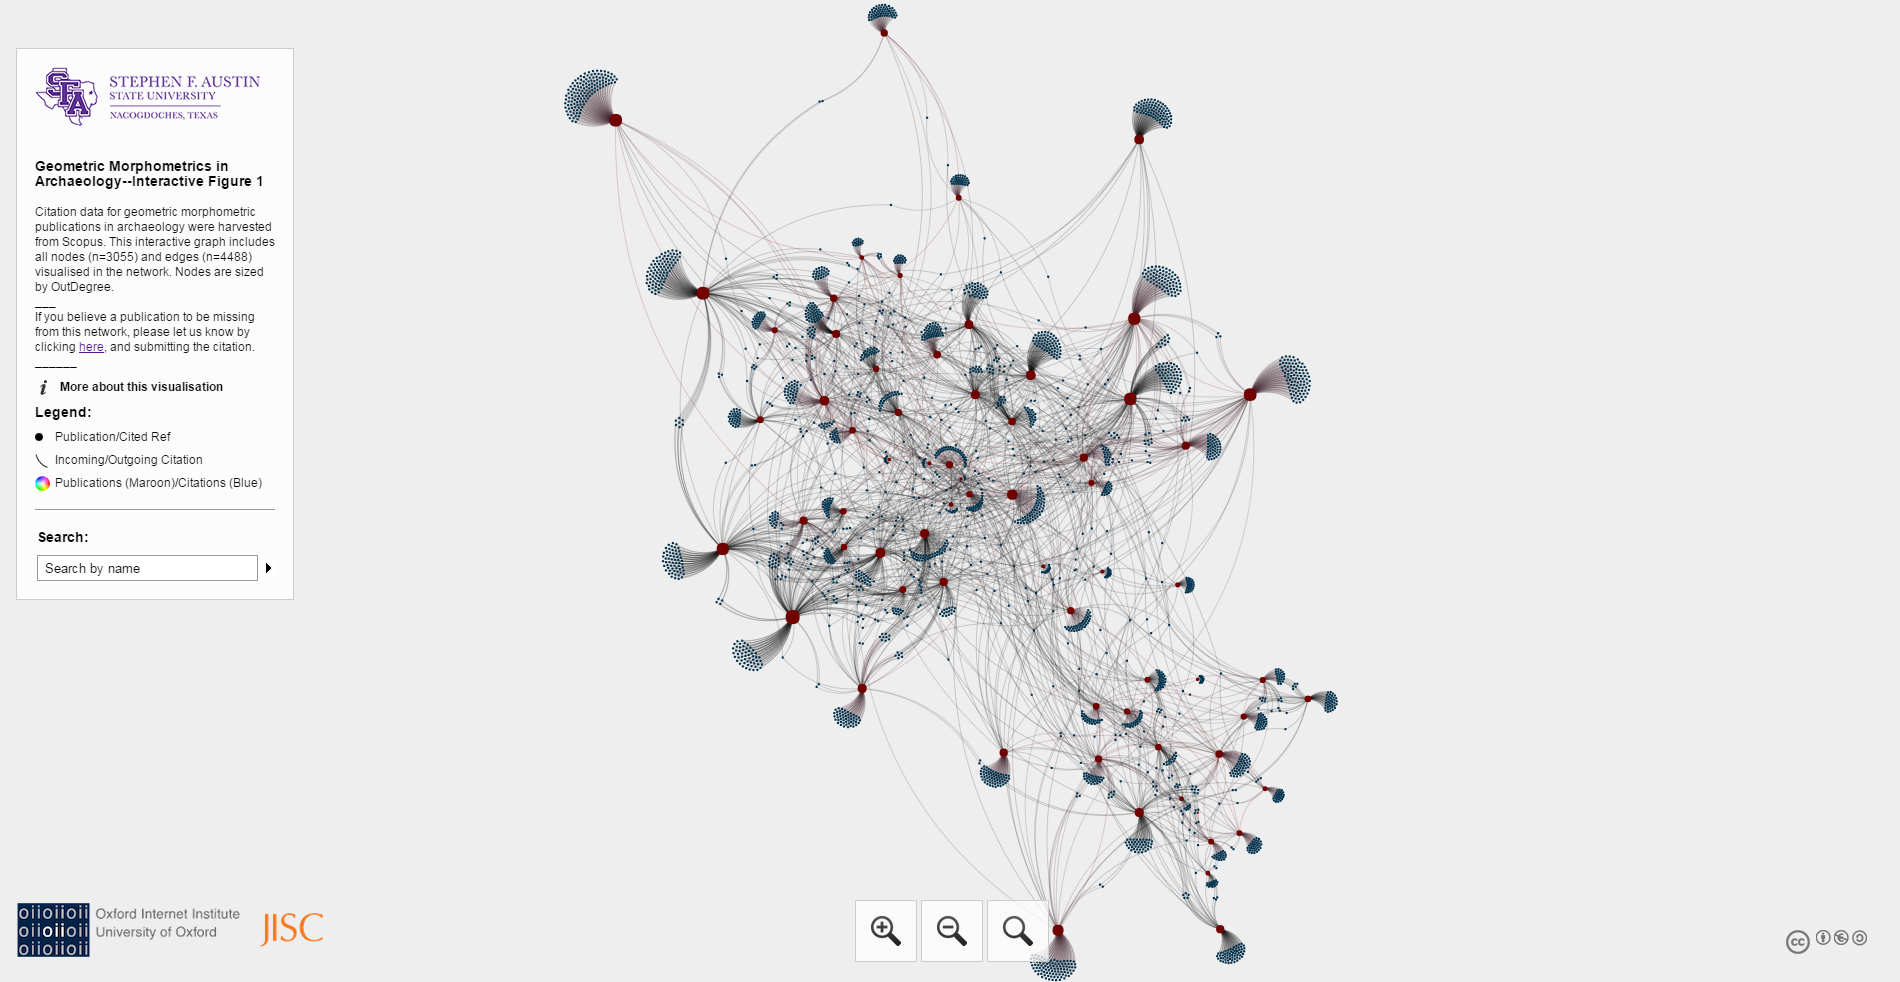
\includegraphics[width=\linewidth]{net}
\caption{Interactive citation network for geometric morphometric studies in archaeology \href{http://crhr-archive.sfasu.edu/GMArchFig1/}{http://crhr-archive.sfasu.edu/GMArchFig1/}.}
\label{fig:network}
\end{figure}

EFA has been increasingly employed in lithic \citep{RN11556,RN4320x,RN11529,RN4350,RN4373,RN4338,RN4353,RN11521} and ceramic analyses  \citep{RN4335}, where analysts continue to develop new approaches that advance archaeological applications \citep{RN4143,RN253,RN11534}. Creative research designs are also being developed and adapted to address some of the very real challenges associated with the oft-fractured and incomplete specimens abundant in the archaeological record \citep{RN11575,RN11574,RN11539,RN11533,RN11730}. These advancements have helped to address challenges with interpretation, while simultaneously aiding in the development of a useful suite of protocols applicable to wide-ranging research questions. 

The more recent fluorescence of landmark-based applications has been driven by advances in anthropology \citep{RN11531,RN1770,RN306,RN1732} and a wide range of other research domains \citep{RN4453,RN1743,RN1762,RN4775,RN11553,RN11535,RN11526,RN11557,RN11554,RN1646,RN11541,RN478,RN11560} that articulate with the rise of the Procrustes paradigm \citep[8]{RN1743}. Archaeological applications have included two-dimensional (2D) analyses of Clovis technology in North America \citep{RN1754,RN1736,RN4378,RN11518,RN11519}, Fishtail or Fell projectile points in South America \citep{RN4346,RN11545}, bifacial points from the Umbu Tradition in Brazil \citep{RN11547,RN370,RN11548}, lanceolate points---\textit{ayampitin}---from Argentina \citep{RN11549}, the size and shape of projectile points from southern Patagonia \citep{RN4338x,RN4337x}, bifacial tools from southern Poland \citep{RN11551}, Final Palaeolithic large tanged points \citep{RN4738}, Paleoindian point types from Florida \citep{RN11528} and the Southern High Plains \citep{RN4358,RN11517}, ceramics from Casas Grandes \citep{RN11631}, flake morphology \citep{RN4334}, and reduction effects \citep{RN4349}; all of which capitalise on the morphological variation that occurs in a single plane \citep{RN1754,RN11542}. 

For research designs that incorporate questions associated with more complex geometry, 3D landmark-based approaches may be more appropriate. Examples from the literature include the development of novel tools and applications \citep{RN1722}, and cover a broad range of artefact categories including projectile points \citep{RN1750,RN1755}, bifaces \citep{RN1727,RN4392,RN11550}, percussive tools \citep{RN1772}, flake scars \citep{RN253}, flake tools \citep{RN11552}, handaxes \citep{RN1730,RN1766,RN3145,RN1733,RN335}, and Caddo ceramics \citep{RN1994}. This study enlists the variation that occurs within a single plane for an aggregated sample of Caddo bottles; however, 3D data were required to identify the widest vessel profile. Additionally, a variety of landmark and semilandmark configurations are in development that will allow for a more robust analysis of 3D morphology associated with specific elements of vessel morphology.

\subsection{Caddo bottles from Louisiana in the Clarence H. Webb collections}

The sample of Caddo bottles used in the analysis (Table ~\ref{tab:Tbl1}) comes from the collections of the late Clarence H. Webb, and were excavated at the Gahagan Mound (16RR1) \citep{RN5274x}, Smithport Landing (16DS4) \citep{RN5270x}, Allen Plantation (16NA6) \citep{RN11778x}, and Belcher Mound (16CD13) \citep{RN5276x,RN5266x} sites in Northwest Louisiana (Figure ~\ref{fig:FigMap}). Some of Webb's collections were previously repatriated to the Caddo Nation of Oklahoma, but many remain in the collections of the Williamson Museum at Northwestern State University, the Louisiana State Exhibit Museum, and the Louisiana State University (LSU) Museum of Natural Science. Caddo ceramic types in the sample include Belcher Engraved (ca. CE 1200-1500) \citep[9, and Plate 5]{RN4302}, Hickory Fine Engraved (ca. CE 500-1000) \citep[71, and Plate 36]{RN4302}, Keno Trailed (ca. CE 1400-1700) \citep[87, and Plate 44]{RN4302}, Smithport Plain (ca. CE 500-1200) \citep[145, and Plate 73]{RN4302}, and Taylor Engraved (ca. CE 1200-1500) \citep[149-151, and Plates 75-76]{RN4302}.

\begin{table}[htbp]\centering
\footnotesize
\caption{Caddo bottles used in the analysis.}
\centering
\begin{tabular}{lccccc}
\toprule
Webb No & Site Name & Trinomial & Context & Museum & Type\\
\midrule
95 & Smithport Landing & 16DS4 & Burial 1 & NSU & Smithport Plain\\
96 & Smithport Landing & 16DS4 & Burial 1 & NSU & Hickory Fine Engraved\\
142 & Allen Plantation & 16NA6 & Unknown & NSU & Hickory Fine Engraved\\
152 & Smithport Landing & 16DS4 & Burial 10 & NSU & Smithport Plain\\
No \# & Smithport Landing & 16DS4? & Unknown & NSU & Hickory Fine Engraved\\
256 & Belcher Mound & 16CD13 & Burial 5 & LSUMNS & Taylor Engraved\\
267 & Belcher Mound & 16CD13 & Burial 5 & LSEM & Belcher Engraved\\
269 & Belcher Mound & 16CD13 & Burial 5 & NSU & Belcher Engraved\\
271 & Belcher Mound & 16CD13 & Burial 5 & LSUMNS & Taylor Engraved\\
361 & Belcher Mound & 16CD13 & Burial 9 & NSU & Belcher Engraved\\
363 & Belcher Mound & 16CD13 & Burial 10 & NSU & Belcher Engraved\\
404 & Belcher Mound & 16CD13 & Burial 11 & NSU & Hickory Fine Engraved\\
405* & Belcher Mound & 16CD13 & Burial 11 & NSU & Smithport Plain\\
430* & Belcher Mound & 16CD13 & Burial 12 & NSU & Smithport Plain\\
775 & Belcher Mound & 16CD13 & Burial 15 & NSU & Belcher Engraved\\
784 & Belcher Mound & 16CD13 & Burial 15 & LSUMNS & Keno Trailed\\
787 & Belcher Mound & 16CD13 & Burial 15 & LSUMNS & Taylor Engraved\\
788 & Belcher Mound & 16CD13 & Burial 15 & NSU & Belcher Engraved\\
803 & Belcher Mound & 16CD13 & Burial 15 & LSUMNS & Belcher Engraved\\
805 & Belcher Mound & 16CD13 & Burial 15 & NSU & Belcher Engraved\\
845 & Belcher Mound & 16CD13 & Burial 17 & NSU & Belcher Engraved\\
852 & Belcher Mound & 16CD13 & Burial 17 & NSU & Keno Trailed\\
897 & Belcher Mound & 16CD13 & House 6 & NSU & Belcher Engraved\\
955 & Gahagan Mound & 16RR1 & Mound A & NSU & Hickory Fine Engraved\\
956 & Gahahan Mound & 16RR1 & Mound A & LSUMNS & Hickory Fine Engraved\\
997 & Belcher Mound & 16CD13 & Burial 24 & NSU & Belcher Engraved\\
1054 & Belcher Mound & 16CD13 & Burial 26 & LSEM & Taylor Engraved\\
1073 & Belcher Mound & 16CD13 & House 6 & NSU & Belcher Engraved\\
\bottomrule
\end{tabular}
\textit{The single vessel (Hickory Fine Engraved) without a Webb number is assumed to have come from the Smithport Landing site in fragments. The bottle was later reassembled, but a number was never assigned. * = only used in the comparison of base/body morphology for Hickory Fine Engraved and Smithport Plain; NSU = Williamson Museum, Northwestern State University; LSUMNS = Louisiana State University Museum of Natural Science; LSEM = Louisiana State Exhibit Museum.}
\label{tab:Tbl1}
\end{table}

\begin{figure}[ht]\centering
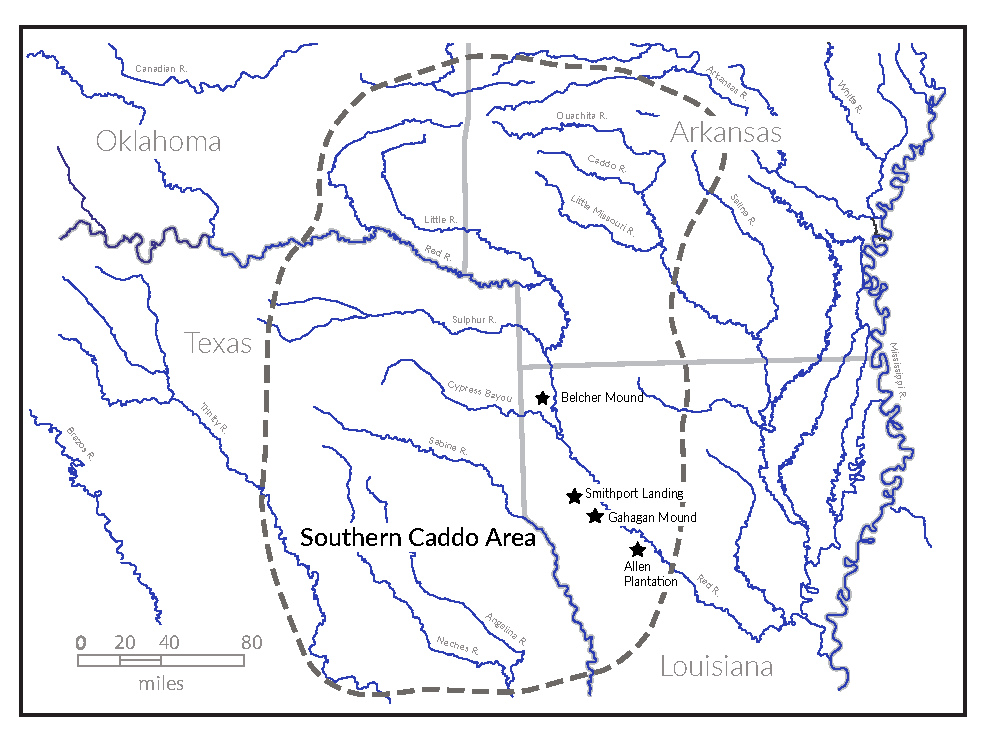
\includegraphics[width=\linewidth]{SCA-LA}
\caption{Locations of the Belcher Mound, Mounds Plantation, Smithport Landing, Gahagan Mound, and Allen Plantation sites in northwest Louisiana.}
\label{fig:FigMap}
\end{figure}

All bottles used in this analysis fall under the purview of the Native American Graves Protection and Repatriation Act (NAGPRA) \citep{RN11778x}, excepting those found in House 6 at the Belcher Mound site (Table ~\ref{tab:Tbl1}). Permission to scan the collection was granted by the Caddo Nation of Oklahoma with the provision that any scan data used in the analysis must not include the texture (colour) file. Full-resolution scan data were forwarded to the Caddo Nation of Oklahoma with the texture applied. This provides the Caddo with an accurate 3D record of each vessel, and a means of viewing a collection that is currently curated across numerous repositories, making it challenging to locate and aggregate.

\section{Methods}

Each of the bottles was scanned with a Creaform GoSCAN 50 at a 0.8 mm resolution in VXelements. Scanner calibration was optimised prior to each scan, with positioning targets required for increased accuracy, and shutter speed reconfigured in each instance. A clipping plane was established to reduce the amount of superfluous data collected during each scan. Following data collection, the resolution of each mesh was increased to 0.5 mm, and the point cloud was transferred to VXmodel where the mesh was rendered following application of the \textit{clean mesh} function, used to remove isolated patches, self-intersections, spikes, small holes, singular vertices, creased edges, narrow triangles, outcropping triangles, narrow bridges, and non-manifold triangles prior to export as an ASCII stl and ASCII ply. The stl functions as a backup, and the ply was subsequently imported to Geomagic Design X (Dx).

\subsection{Alignment and reference geometry}

Following the transfer to Dx, each mesh was subjected to a second quality check to eliminate non-manifold poly-vertices, folded poly-faces, dangling poly-faces, small clusters, small poly-faces, non-manifold poly-faces, crossing poly-faces, and small tunnels. Due to the paucity of homologous landmarks on cultural artefacts \citep{RN1730}, reference geometry was constructed in and around each vessel in a manner that yields a replicable configuration of nine landmarks, and 46 equidistant semilandmarks along the widest vessel profile, with notable similarities to previous landmark configurations used by \citet[Figure 4]{RN1752}, \citet[Figure 5]{RN1994}, and \citet[Figure 4]{RN11631}. 

The first component of reference geometry added, and principal assumption, was a reference vector. A sampling ratio of 100 percent was used to apply the reference vector on a revolving axis, after which a reference point was added by projecting it atop the mesh surface at the location where the reference vector exits the base of the vessel. A reference plane was inserted using the \textit{pick multiple points} function, by adding a series of 10 points around the circumference of the bottle's base. Each element of reference geometry (vector, point, and plane) was then used in an interactive 3-2-1 alignment where the vessel was aligned to a global origin, orienting it in 3D space where it sits upright atop a planar surface (assumed to be the intent of the maker). Following alignment, the reference plane and point were deleted.

The widest profile was defined as the location on the mesh that lies farthest from that point where the reference vector exits the base while oriented atop the planar surface. To identify that location, a mesh sketch was generated with the planar method using the plane at the base of the vessel to identify and sketch the widest vessel circumference. By using the plane at the base of the vessel for the sketch, the point at which the reference vector exits the mesh remains linked to the remainder of the reference geometry. A circle is then sketched using the vector as the centre, extending outward until the whole of the vessel fits within. Using the mesh sketch, a cylinder (surface) is extruded around the vessel. The \textit{accuracy analyser} in Dx is then used to identify the point on the vessel with the lowest deviation from the extruded surface, and a plane (MPlane) is inserted coplanar to the vector and oriented to the widest point, bisecting the vessel at the widest profile.

Using the MPlane as the basis for a second mesh sketch, a spline with 15 interpolation points was sketched on one rim. Above that sketch, a horizontal line was added, then both were used to determine the horizontal tangent of the rim. A vertical line was subsequently added that bisects the rim at the location of the tangent. This operation was repeated for the opposing rim. The logic behind this added step is that the surface scanner cannot reach the interior of the vessel, so the spline needed to be cut in a replicable location. For vessels with a direct (vertical) rim, the preceding step was extended to include one additional measure. A line was drawn between each tangent, then a second from the intersection of the line and reference vector to a point 10 mm down the vector, where a horizontal line---parallel with the rim peaks---was inserted that intersects with both external walls of the vessel. It is at this intersection that the final mesh sketch was cut to discriminate between the neck and rim.

Using the MPlane as the basis for a third sketch, a spline was populated for the entirety of the silhouetted profile. That spline was split at the horizontal tangent on each rim, and the remaining sections that continued into the bottle interior were deleted. The second split was added at the intersection of the spline and reference vector (centre of base). Four additional splits were added at the juncture of the base/body and body/neck on each side of the vessel at the points of highest curvature. For those bottles with everted rims, the spline was cut at the point of highest curvature between the rim and neck; for those with direct rims, the spline was cut at the intersection of the horizontal line identified in the previous step. The point of highest curvature used to split the spline was identified using the \textit{curvature} function in Dx, and does not represent an arbitrary location.

\subsection{Landmarks and semilandmarks}

A total of nine landmarks (Table ~\ref{tab:Tbl3}) and 46 semilandmarks divide each bottle into four discrete components corresponding with the rim, neck, body, and base (Figure ~\ref{fig:Fig1a-845}). Landmarks and semilandmarks are populated along the spline, always beginning on the side of the profile determined to include the widest point. Divisions between each component articulate with those of the spline splits identified in the previous section, and are based upon specific geometric features where landmarks were placed at each of the points in Table ~\ref{tab:Tbl3} with a series of equidistant semilandmarks between. 

\begin{figure}[htbp]\centering
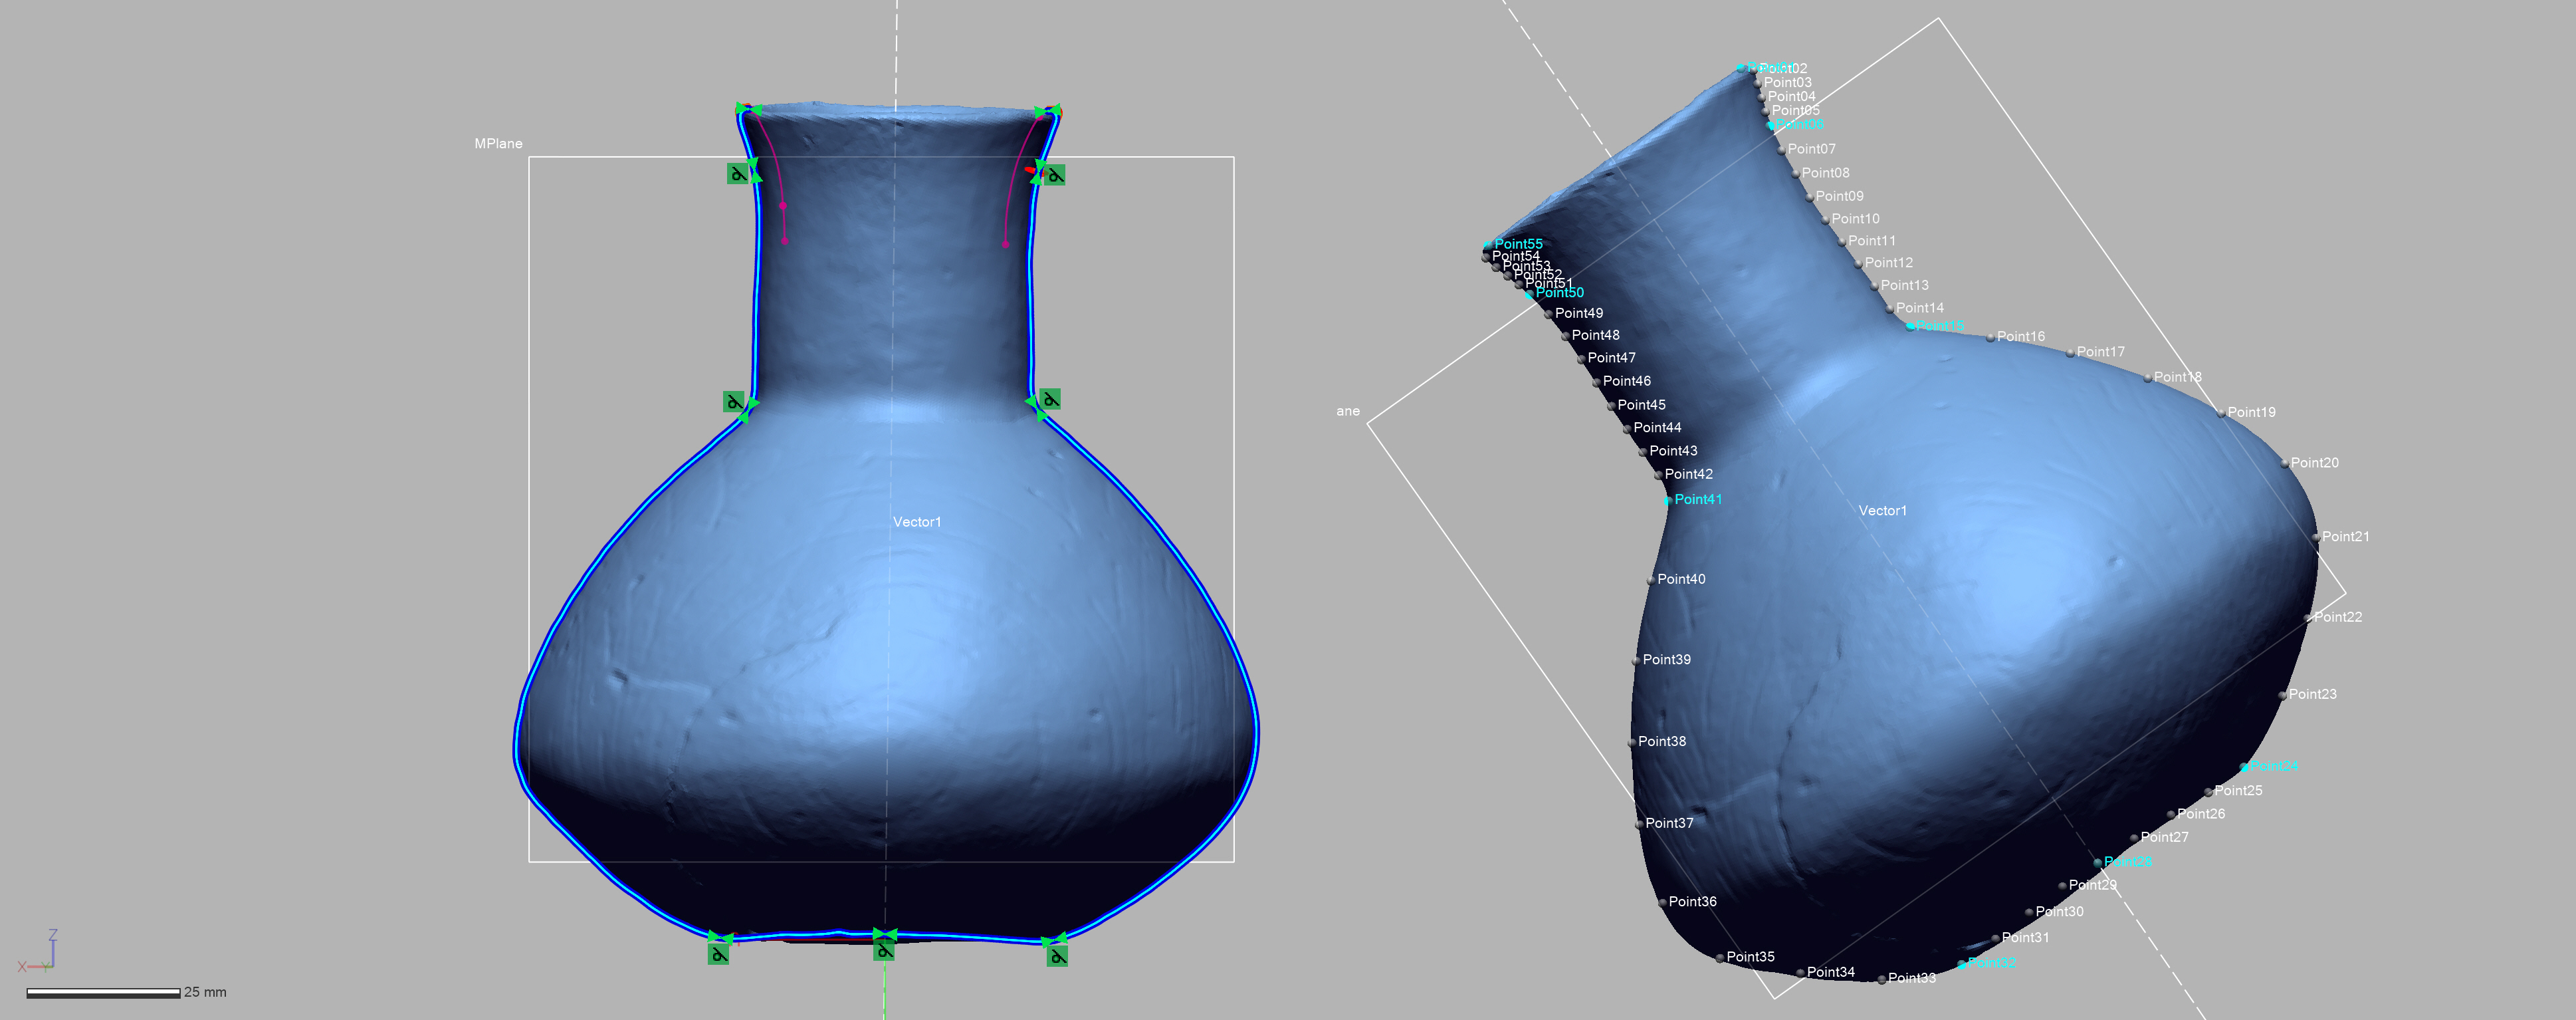
\includegraphics[width=\linewidth]{FigSSLM}
\caption{Spline splits for discrete components (rim, neck, body, and base) used in the GM analysis (left) segregated by landmarks (blue), with equidistant semilandmarks (white) populated between (right).}
\label{fig:Fig1a-845}
\end{figure}

\begin{table}[htbp]\centering
\footnotesize
\caption{Landmarks used in this analysis.}
\centering
\begin{tabular}{lcp{7.5cm}}
\toprule
Landmark & Location & Definition\\
\midrule
Point01 & Rim peak & Horizontal tangent of rim curvature on widest side of vessel\\
Point06 & Rim/Neck & Point of highest curvature (everted rim) or intersection of horizontal line 10 mm below rim tangents (direct rim)\\
Point15 & Neck/Body & Point of highest curvature\\
Point24 & Body/Base & Point of highest curvature\\
Point28 & CentreBase & Intersection of vector and external surface of 3D mesh.\\
Point32 & Body/Base & Point of highest curvature\\
Point41 & Neck/Body & Point of highest curvature\\
Point50 & Rim/Neck & Point of highest curvature (everted rim) or intersection of horizontal line 10 mm below rim tangents (direct rim)\\
Point55 & Rim peak & Horizontal tangent of rim curvature\\
\bottomrule
\end{tabular}
\label{tab:Tbl3}
\end{table}

While sliding semilandmarks were an early consideration of this research design, the choice to use equidistant semilandmarks rather than sliding semilandmarks is based upon results from an earlier iteration of this analysis (Figure ~\ref{fig:slide}). The first landmark and sliding semilandmark configuration did not split the spline between the neck and rim, and when mean shapes were generated for each type, an anomaly (from the everted rims of the Belcher Engraved bottles) was added to the otherwise direct or tapered necks of the Hickory Fine Engraved and Smithport Plain bottles. Given that the use of sliding semilandmarks could potentially influence the  results of this analysis by adding a component of morphology to specimens where it does not exist, they were abandoned.

\begin{figure}[ht]\centering
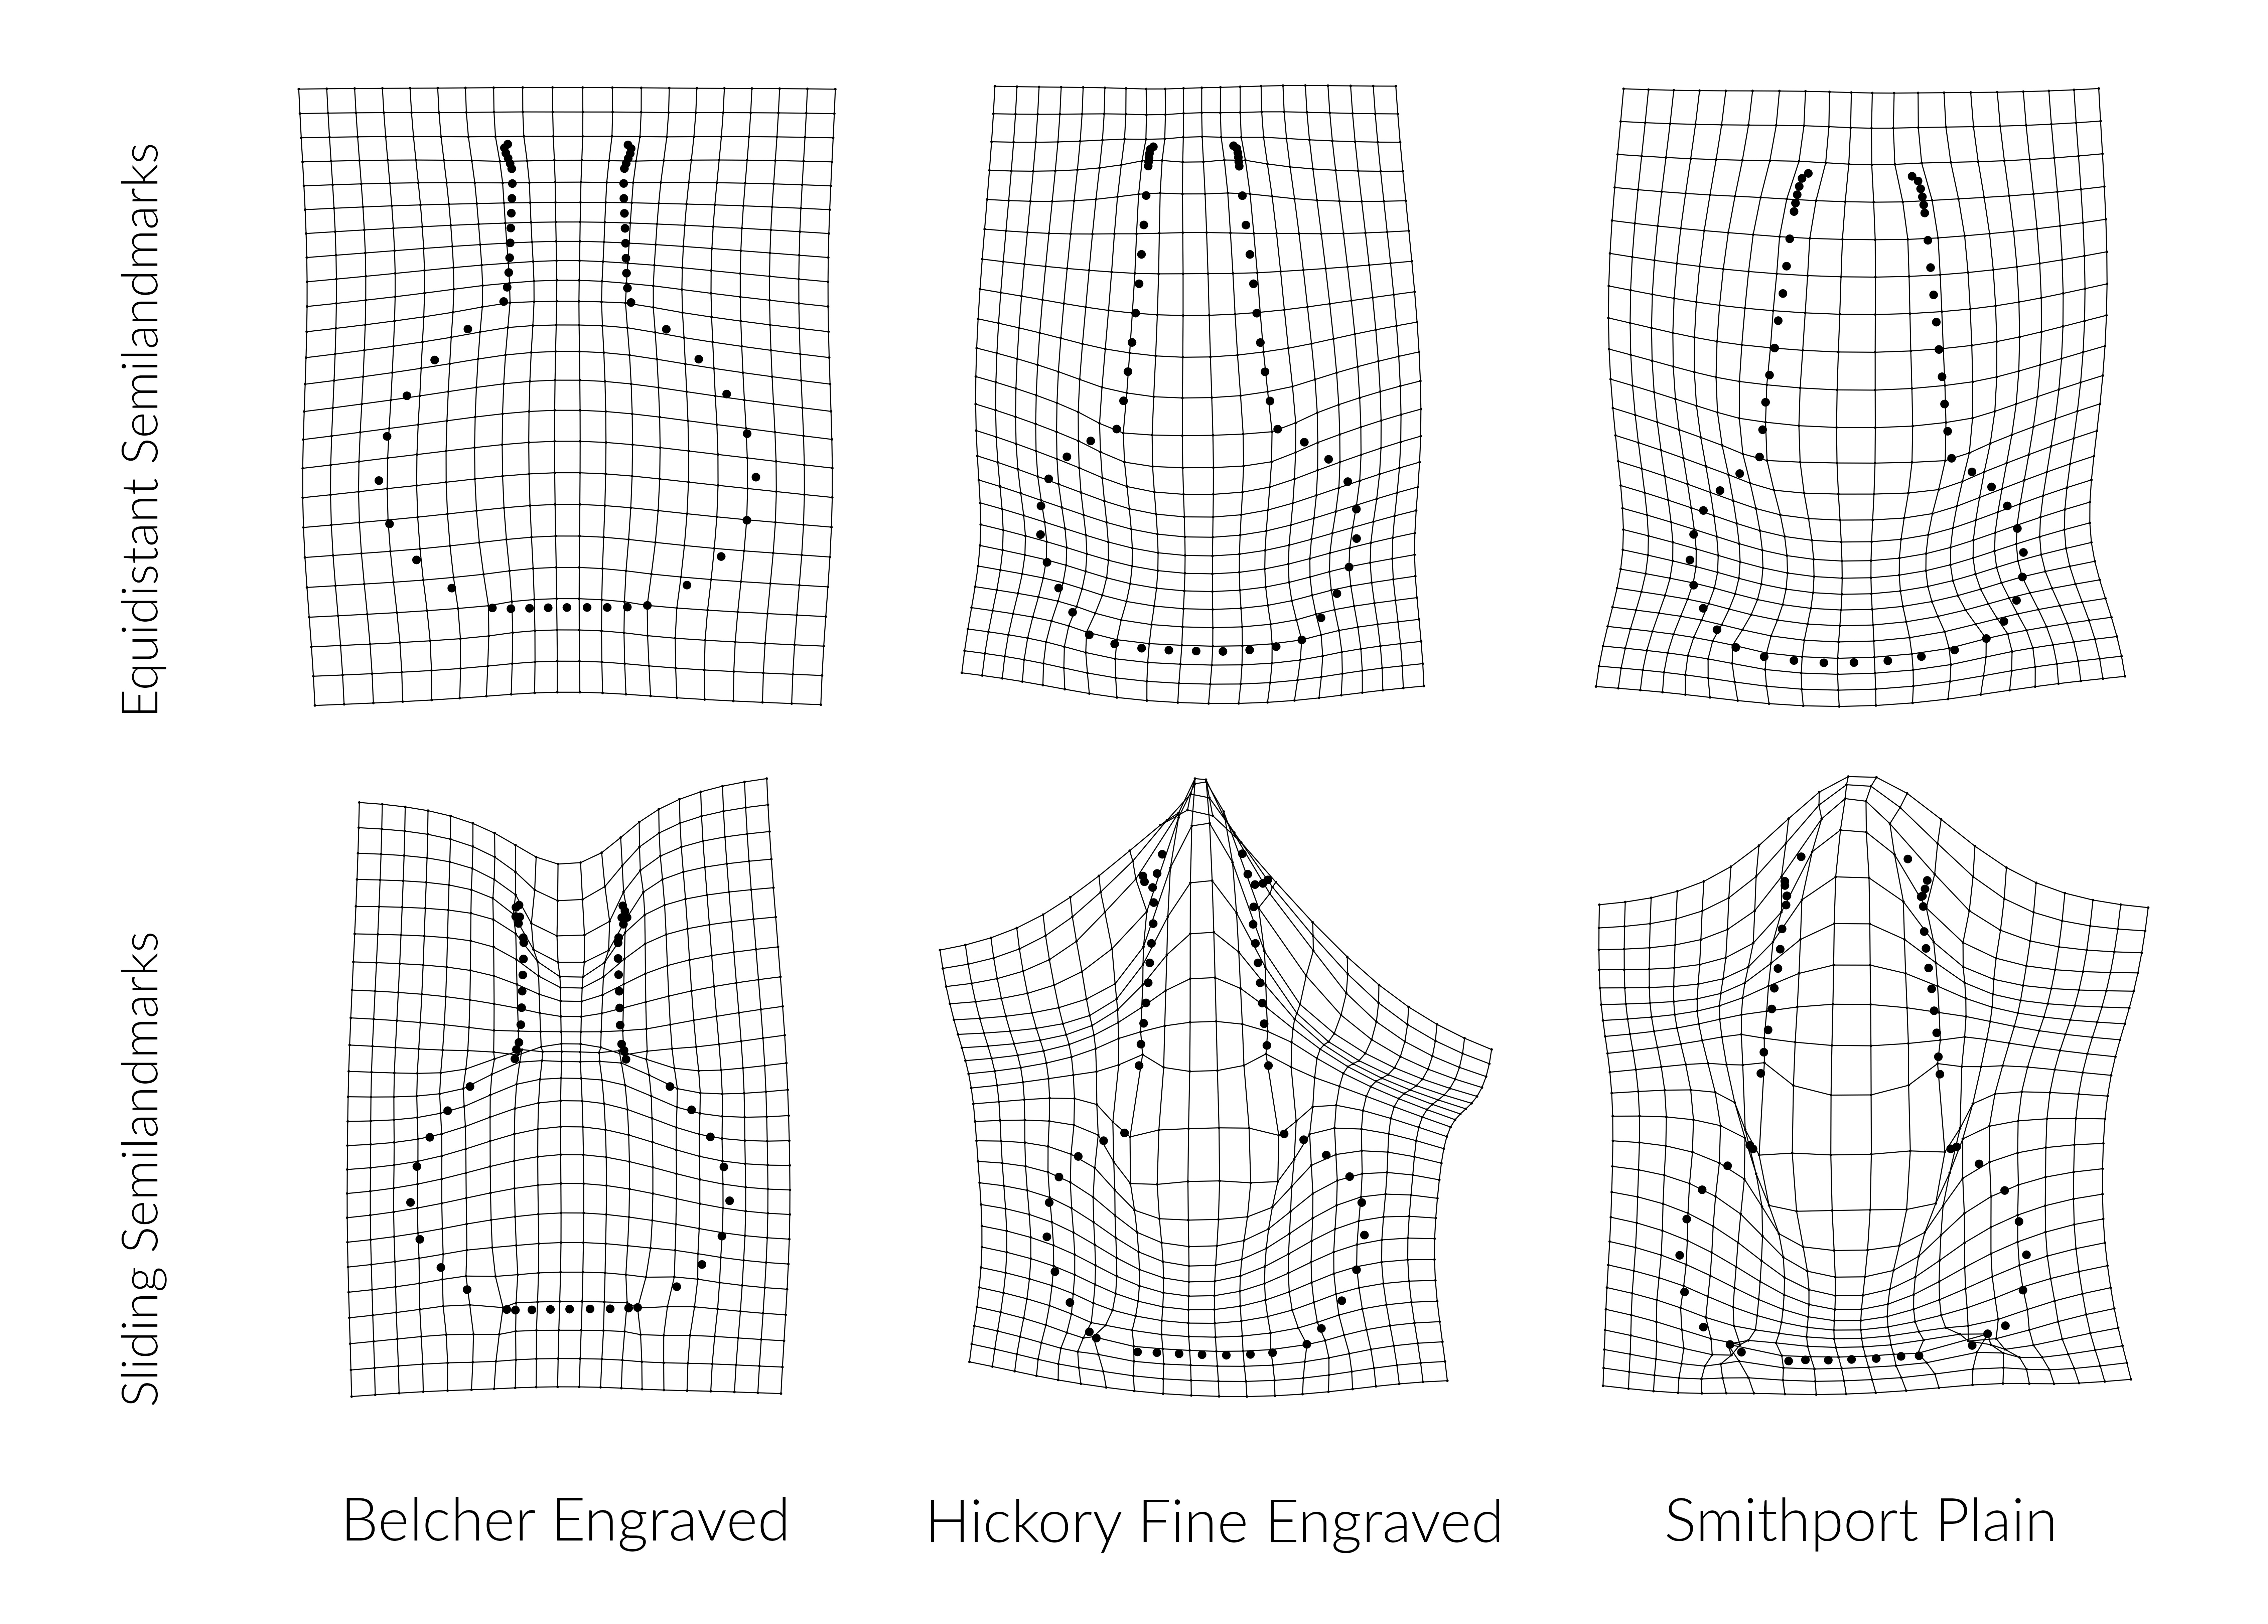
\includegraphics[width=\linewidth]{slide}
\caption{Mean consensus configurations for landmarks and equidistant semilandmarks (final analysis; top) and sliding semilandmarks (earlier iteration of analysis; bottom) associated with the Belcher Engraved, Hickory Fine Engraved (HFE), and Smithport Plain (SMPL) types that illustrate a morphological anomaly added to the HFE and SMPL bottles near the rim.}
\label{fig:slide}
\end{figure}

\subsection{Analysis}

Landmarks and equidistant semilandmarks were exported as x,y and z coordinate data from Dx. Those data were aligned to a global coordinate system \citep{RN11622,RN11623,RN11563}, achieved through generalised Procrustes superimposition \citep{RN478} performed in R 3.5.0 \citep{R} using the \textit{geomorph} library v.3.0.6 \citep{RN11530,RN1774}. Procrustes superimposition translates, scales, and rotates the coordinate data to allow for comparisons among objects \citep{RN11564,RN478}. The \textit{geomorph} package uses a partial Procrustes superimposition that projects the aligned specimens into tangent space subsequent to alignment in preparation for the use of multivariate methods that assume linear space \citep{RN1646,RN11563}.

Principal Components Analysis \citep{RN1746} was used to visualise shape variation among the vessel types. The shape changes described by each principal axis are commonly visualised by using thin-plate spline warping of a reference 3D mesh \citep{RN1731,RN479}. A residual randomisation permutation procedure (RRPP; n=1000 permutations) was used for all Procrustes ANOVAs \citep{RN1655,RN11775}, which has higher statistical power and a greater ability to identify patterns in the data should they be present \citep{RN1719}. To assess whether shape changes with size (allometry), and differs by group (types and sites), Procrustes ANOVAs \citep{RN1749} were run that also enlist effect-sizes (z-scores) computed as standard deviates of the generated sampling distributions \citep{RN1756}. In addition to the Procrustes ANOVA run to assess whether shape changes with size, the assumption of allometric slope homogeneity was tested with the \textit{procD.allometry} function using the PredLine option \citep{RN1649}. Should this test not be significant, then allometric slopes are similar---if not identical---across temporal ranges and types, tested separately.

A Procrustes ANOVA and pairwise test was used to identify sites where bottle shapes differ. The pairwise test is conceptually similar to trajectory analysis \citep{RN11573,RN1648,RN1776,RN1739} in that pairwise statistics are vector lengths between vectors, but differs since a factorial model is not explicitly needed to contrast vectors between point factor levels nested within group factor levels \citep{RN11530}. Procrustes variance was used to discriminate between groups and compare the amount of shape variation (morphological disparity) across sites \citep{RN11560}, which  is estimated as the Procrustes variance using residuals of linear model fit \citep{RN11530}. For the sample of whole vessels, a pairwise comparison of morphological integration was used to test the strength of integration between the four components using a z-score \citep{RN11700}.

\section{Results}

The mean consensus configuration and Procrustes residuals were calculated using a Generalised Procrustes Analysis (GPA) for the aggregated sample \citep[Figure 3]{RN1720} (Figure ~\ref{fig:FigGPA}). This initial view of the data demonstrates the degree of variability in Caddo bottles that occurs across the sample. As an exploratory measure, GM methods---to include GPA---aid in clarifying shape differences, and in the production of novel \textit{a posteriori} hypotheses \citep{RN1720}.

\begin{figure}[htbp]\centering
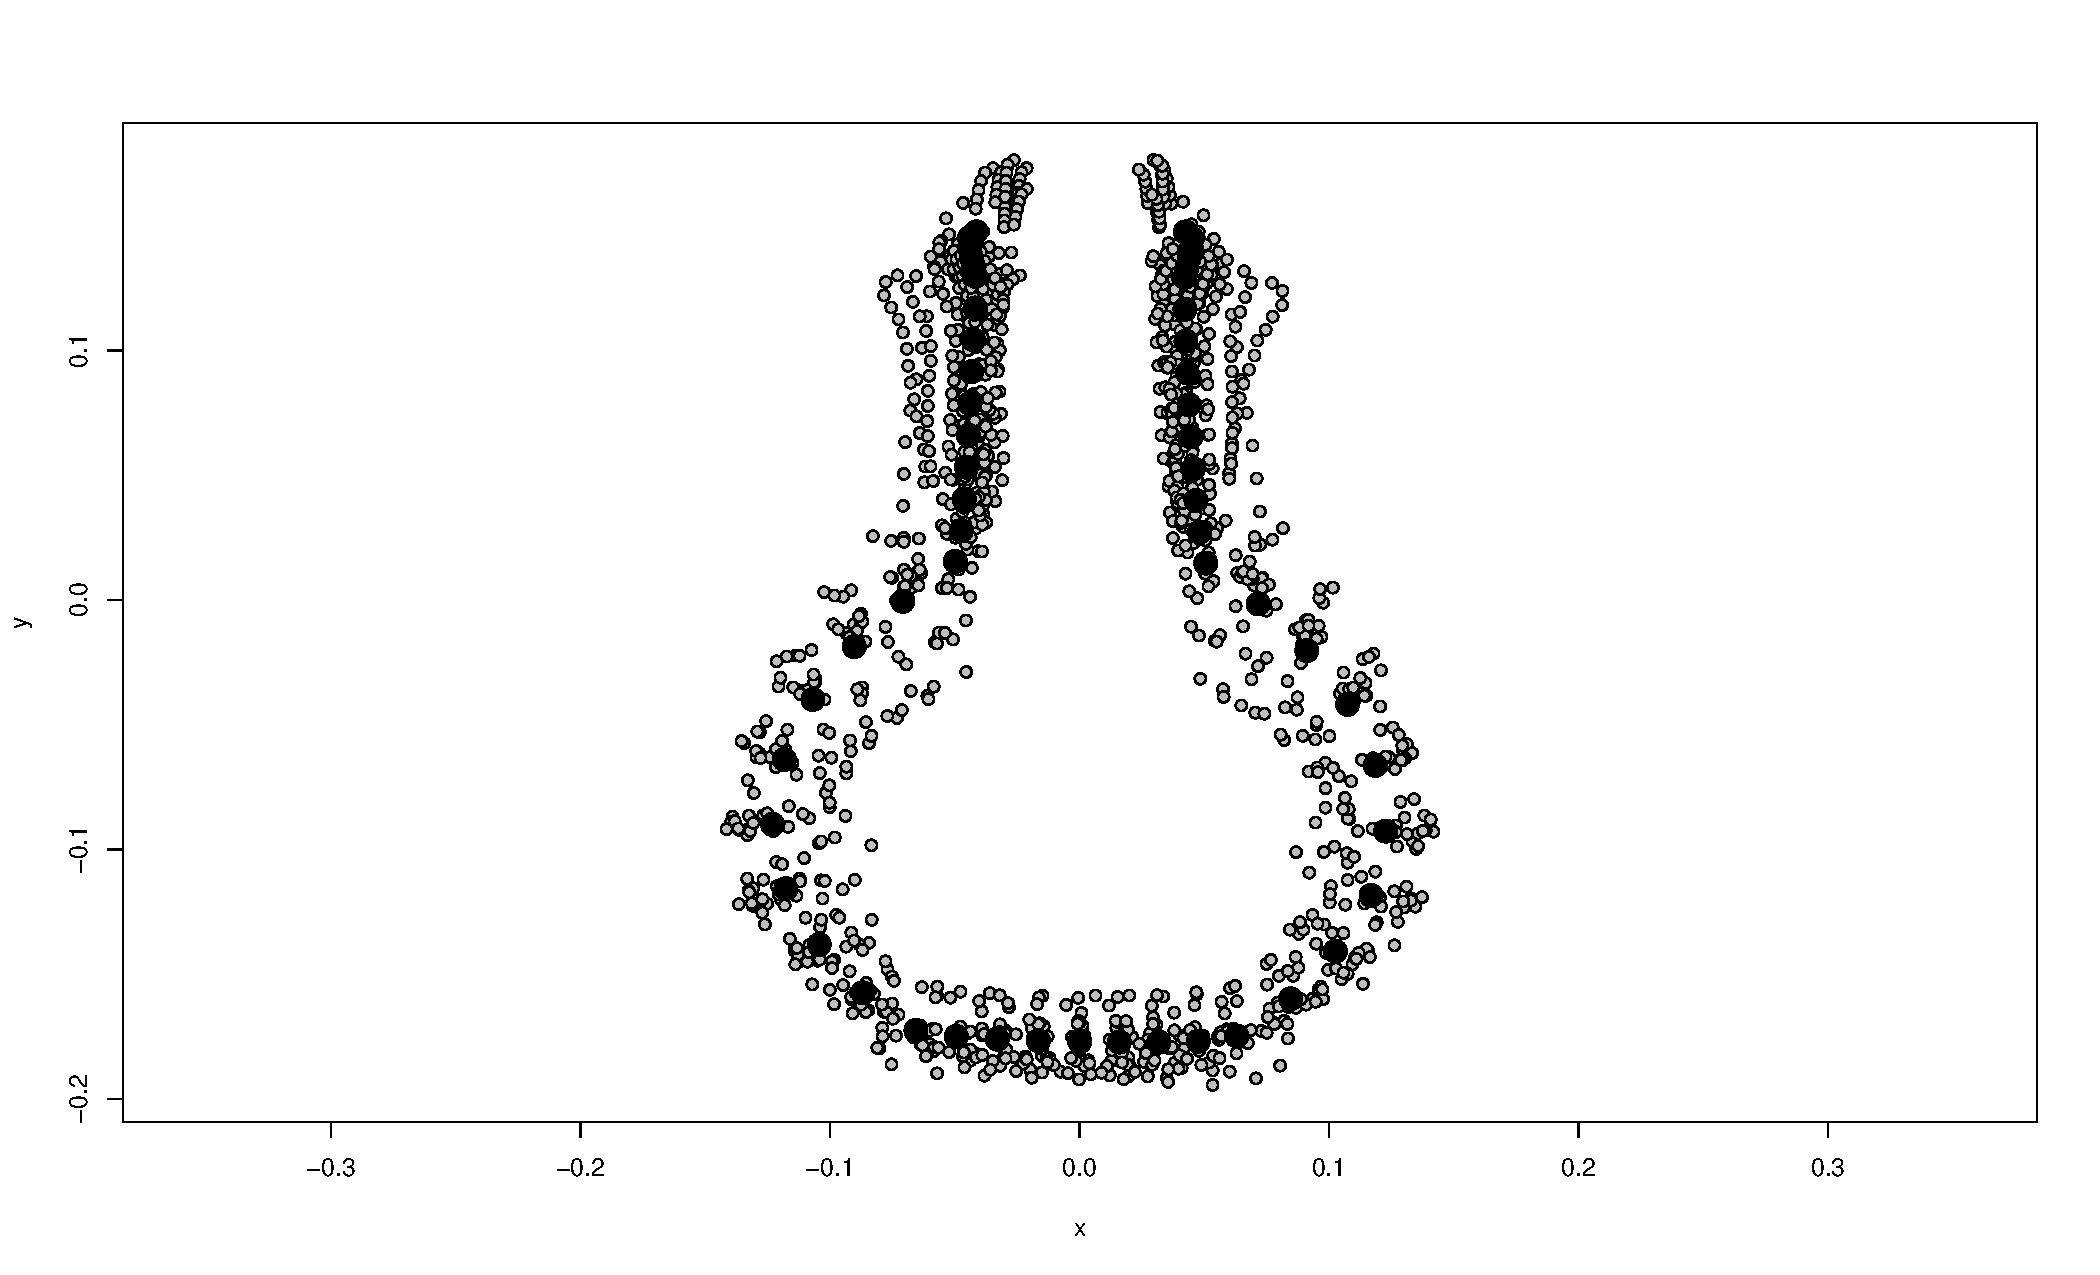
\includegraphics[width=\linewidth]{gpa-all}
\caption{Results of Generalised Procrustes Analysis. Mean consensus configuration shown in black; samples in gray.}
\label{fig:FigGPA}
\end{figure}

Principal components analysis (PCA) was conducted on scaled, translated, and rotated landmarks, and demonstrate that the first two PCs account for 63 (PC1) and 22 (PC2) percent of the variation in bottle shape (Table ~\ref{tab:Tblpca1} and Figure ~\ref{fig:FigPCA}). Together, PC1 and PC2 account for 85 percent of shape variation for Caddo bottles, with all remaining PCs representing less than eight percent of the variation (Table ~\ref{tab:Tblpca1}). The first two PCs are plotted in Figure ~\ref{fig:FigPCA}, where warp grids represent the shape changes along PC1. This plot indicates that shape changes associated with PC1 articulate most readily with neck and body shape. Those shape changes associated with PC2 are dominated by differences in bottle height.

\begin{table}[htbp]\centering
\footnotesize
\caption{Results of principal components analysis for first 10 PCs (> 99 percent of total variance explained).}
\centering
\begin{tabular}{lp{2cm}p{2cm}p{2cm}}
\toprule
 & SD & PVE & CVE\\
\midrule
PC1 & 0.1028 & 0.6281 & 0.6281\\
PC2 & 0.0608 & 0.2197 & 0.8478\\
PC3 & 0.03666 & 0.07989 & 0.92769\\
PC4 & 0.02242 & 0.02988 & 0.95756\\
PC5 & 0.01587 & 0.01497 & 0.097253\\
PC6 & 0.01294 & 0.00995 & 0.98248\\
PC7 & 0.009728 & 0.005630 & 0.988110\\
PC8 & 0.007619 & 0.003450 & 0.991560\\
PC9 & 0.006415 & 0.002450 & 0.994010\\
PC10 & 0.005605 & 0.001870 & 0.995870\\
\bottomrule
\end{tabular}
\smallskip\\
SD - standard deviation; PVE - percentage variance explained; CVE - cumulative variance explained.
\label{tab:Tblpca1}
\end{table}

\begin{figure}[htbp]\centering
\includegraphics[width=\linewidth]{pcacomp}
\caption{Results of PCA summarising shape variation by type.}
\label{fig:FigPCA}
\end{figure}

A Procrustes ANOVA was used to test for allometry, and results do indicate significant allometry in this sample (RRPP = 1000; Rsq = 0.27661; Pr(>F) = 0.001). Plots of predicted allometric trajectories for temporal (Formative-Early and Late-Historic) and type factors are presented in Figure ~\ref{fig:FigAllometry}. The allometric trajectory of Formative-Early Caddo bottles (Hickory Fine Engraved and Smithport Plain) differs significantly (RRPP = 1000; Rsq = 0.06143; Pr(>F) = 0.001) from that of Late-Historic Caddo bottles (Belcher Engraved, Keno Trailed, and Taylor Engraved) as they increase in size (Figure ~\ref{fig:FigAllometry}). Allometric trajectories also differ significantly by type (RRPP = 1000; Rsq = 0.13450; Pr(>F) = 0.001) (Figure ~\ref{fig:FigAllometry}), and the size of the Formative-Early bottles, specifically those of the Hickory Fine Engraved type, extends beyond the range of the Late-Historic types.

\begin{figure}[htbp]\centering
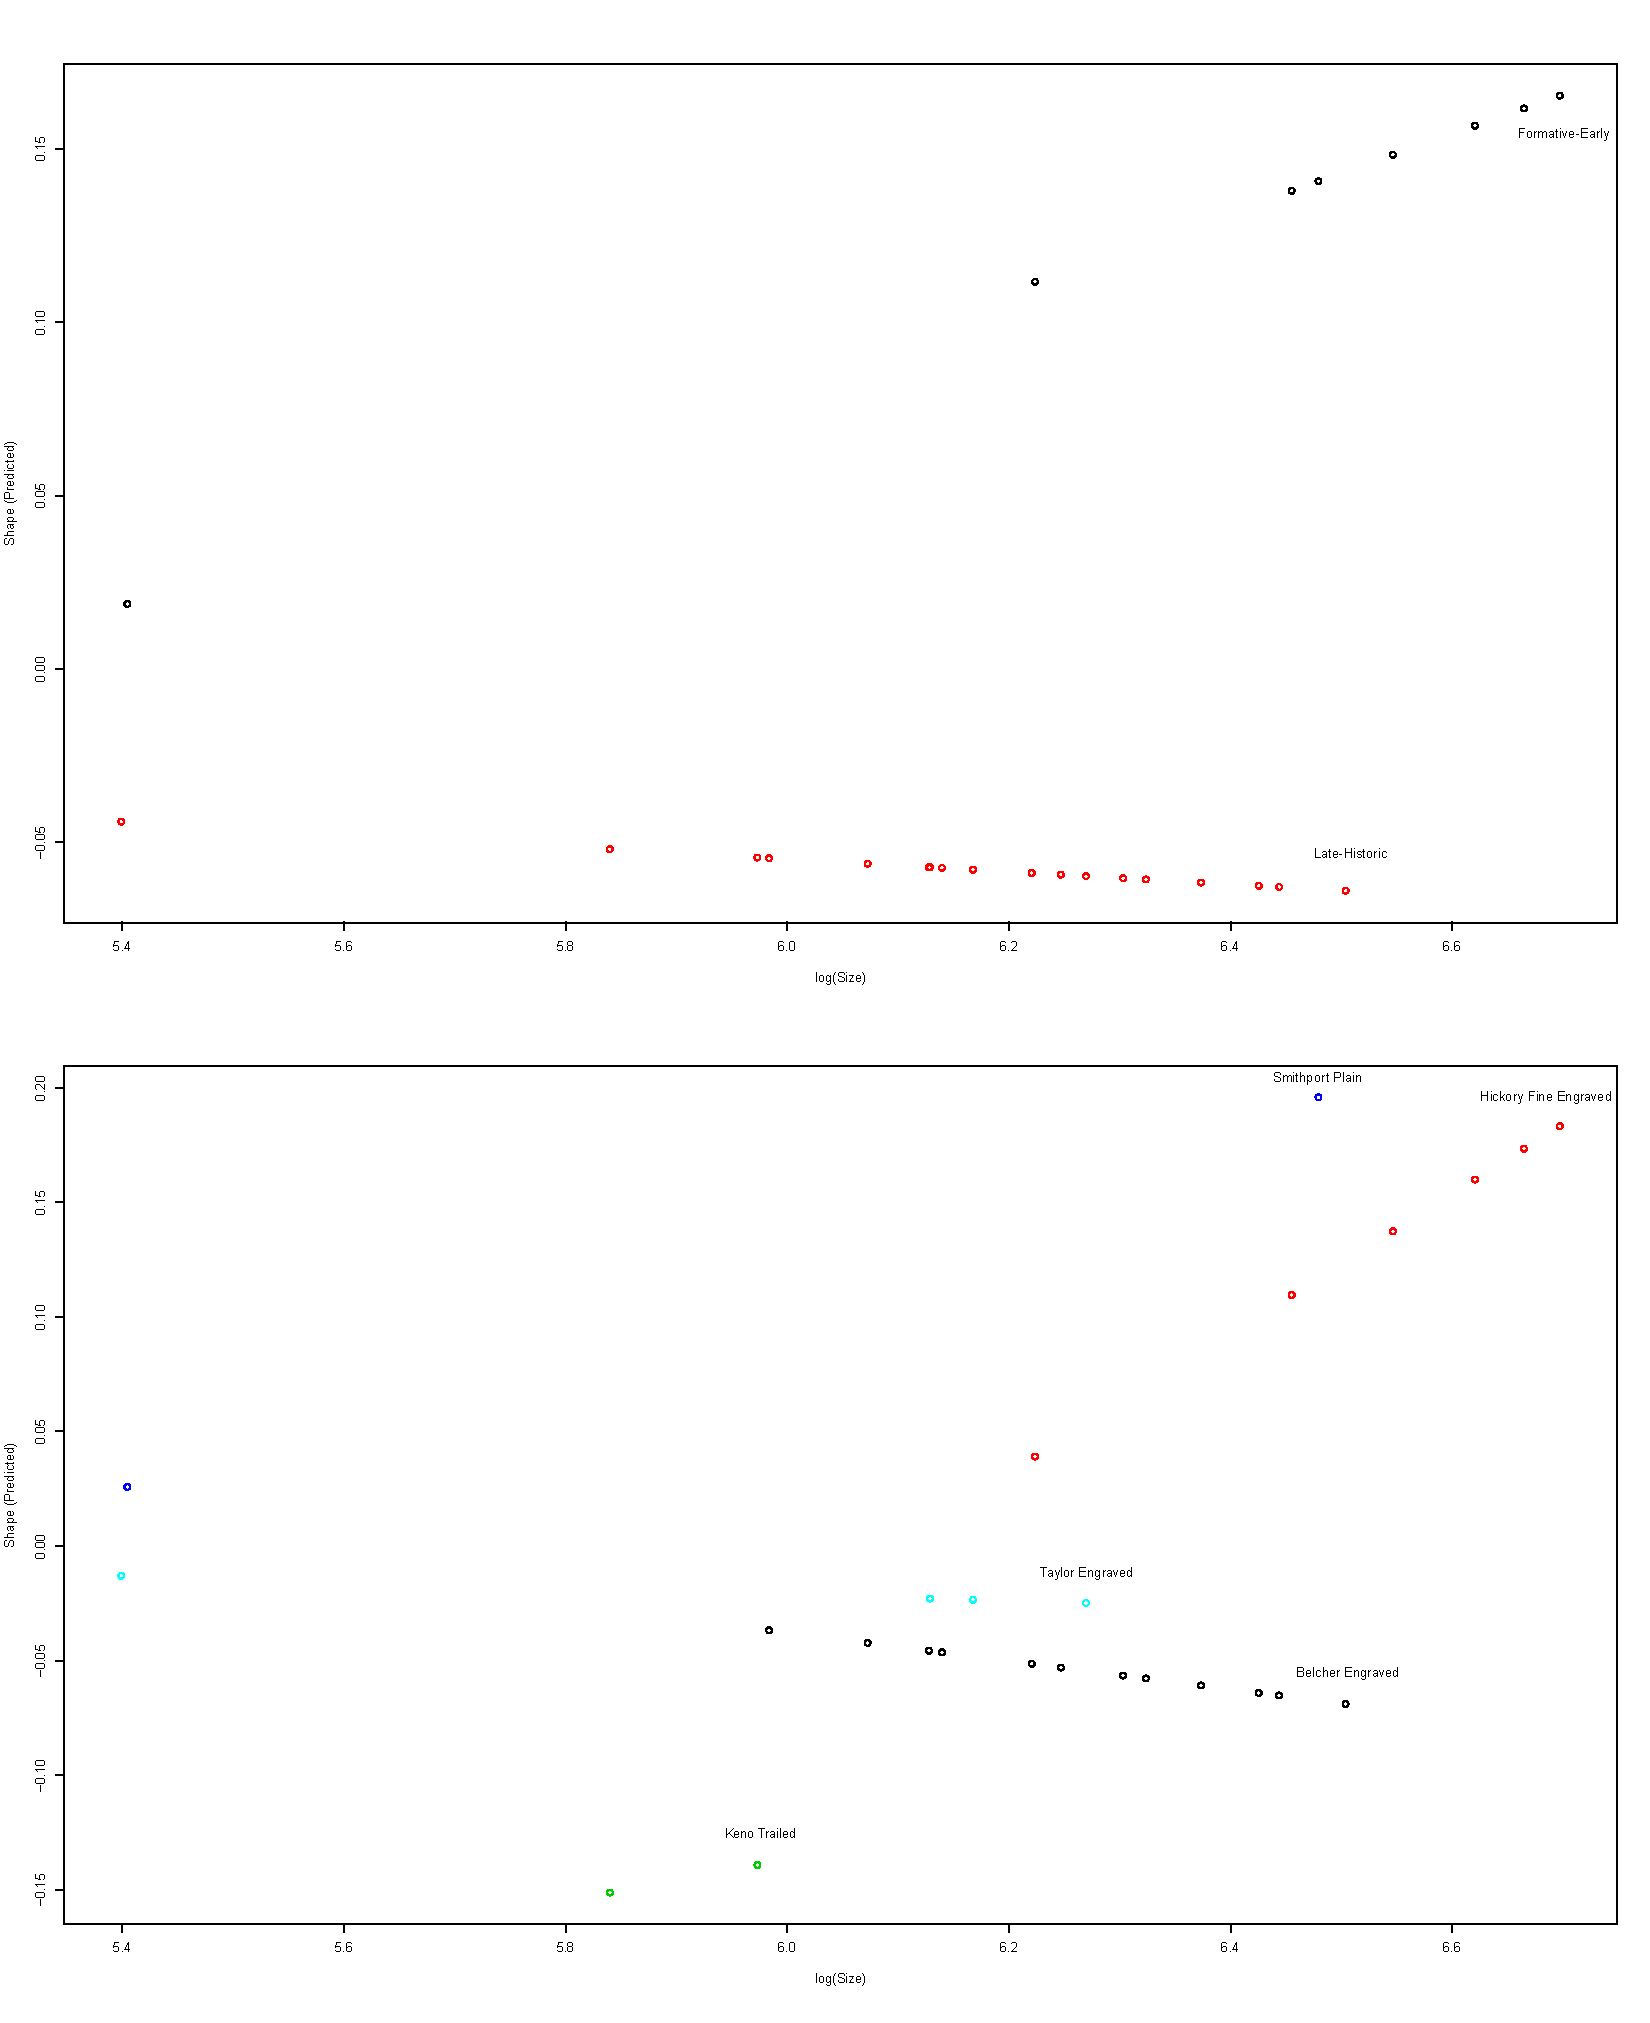
\includegraphics[width=\linewidth]{allometry}
\caption{Predicted values of Caddo bottle shape from temporal (top) and type (bottom) regressions versus log(Centroid Size).}
\label{fig:FigAllometry}
\end{figure}

A Procrustes ANOVA was used to test for a significant difference in bottle shape by site. Results of the ANOVA indicate a significant difference in bottle shape by site (RRPP = 1000; Rsq = 0.6593; Pr(>F) = 0.001). A pairwise test of shapes was subsequently conducted for groups designated by site. Results confirm a significant difference in bottle shape at the Belcher Mound site when compared with Gahagan Mound and Smithport Landing (Table ~\ref{tab:Tbl3x}).

\begin{table}[htbp]\centering
\footnotesize
\caption{P-values and effect sizes for advanced Procrustes ANOVA and pairwise test (RRPP = 1000) of shape by site.}
\centering
\begin{tabular}{lrrrr}
\toprule
 & Allen Pl & Belcher Md & Gahagan Md & Smithport Lnd\\
\midrule
Allen Plantation & 1.000 & 0.229 & 0.715 & 0.780\\
 & (0.0000000) & (1.052018) & (-0.68433097) & (-0.87399319)\\
Belcher Mound & 0.229 & 1.000 & \textbf{0.001} & \textbf{0.001}\\
 & (1.0520179) & (0.000000) & (4.30912352) & (4.69094927)\\
Gahagan Mound & 0.715 & \textbf{0.001} & 1.000 & 0.455\\
 & (-0.6843310) & (4.309124) & (0.00000000) & (-0.02297927)\\
Smithport Landing & 0.780 & \textbf{0.001} & 0.455 & 1.000\\
 & (-0.8739932) & (4.690949) & (-0.02297927) & (0.00000000)\\
\bottomrule
\end{tabular}\\
\smallskip
\textit{Significant results in bold; effect sizes (z) listed in parentheses.}
\label{tab:Tbl3x}
\end{table}

A second pairwise test of shapes was conducted for groups designated by bottle types (Table ~\ref{tab:Tbltypex} and Figure ~\ref{fig:FigMean}). Results indicate that Belcher Engraved bottle shape differs significantly from  Hickory Fine Engraved, Keno Trailed, and Smithport Plain bottle shape. Taylor Engraved bottles only differ significantly from Hickory Fine Engraved bottle shape, which differ significantly from Belcher Engraved and Keno Trailed. The two Formative-Early Caddo bottle types thus express similarities in shape. The Belcher Engraved and Taylor Engraved bottles from the Late-Historic Caddo period do not differ significantly, and include similar bottle shapes with divergent allometric trajectories as vessel size increases (Figure ~\ref{fig:FigAllometry}).

\begin{table}[htbp]\centering
\footnotesize
\caption{P-values and effect sizes for advanced Procrustes ANOVA and pairwise test (RRPP = 1000) of shape by type.}
\centering
\begin{tabular}{lrrrrr}
\toprule
 & Belcher Eng & Hickory FE & Keno Tr & Smithport Pl & Taylor Eng\\
\midrule
Belcher Eng & 1.000 & \textbf{0.001 }& \textbf{0.041} & \textbf{0.006} & 0.757\\
 & (0.0000000) & (5.0753316) & (2.158402) & (3.3304742) & (-0.7706873)\\
Hickory FE & \textbf{0.001} & 1.000 & \textbf{0.001} & 0.282 & \textbf{0.018}\\
 & (5.0753316) & (0.0000000) & (4.975588) & (0.4314228) & (2.5527396)\\
Keno Tr & \textbf{0.041} & \textbf{0.001} & 1.000 & \textbf{0.012} & 0.065\\
 & (2.1584018) & (4.9755878) & (0.000000) & (2.8096335) & (1.6590595)\\
Smithport Pl & \textbf{0.006} & 0.282 & \textbf{0.012} & 1.000 & 0.063\\
 & (3.3304742) & (0.4314228) & (2.809633) & (0.0000000) & (1.7108783)\\
Taylor Eng & 0.757 & \textbf{0.018} & 0.065 & 0.063 & 1.000\\
 & (-0.7706873) & (2.5527396) & (1.659059) & (1.7108783) & (0.0000000)\\
\bottomrule
\end{tabular}\\
\smallskip
\textit{Significant results in bold; effect sizes (z) listed in parentheses.}
\label{tab:Tbltypex}
\end{table}

\begin{figure}[ht]\centering
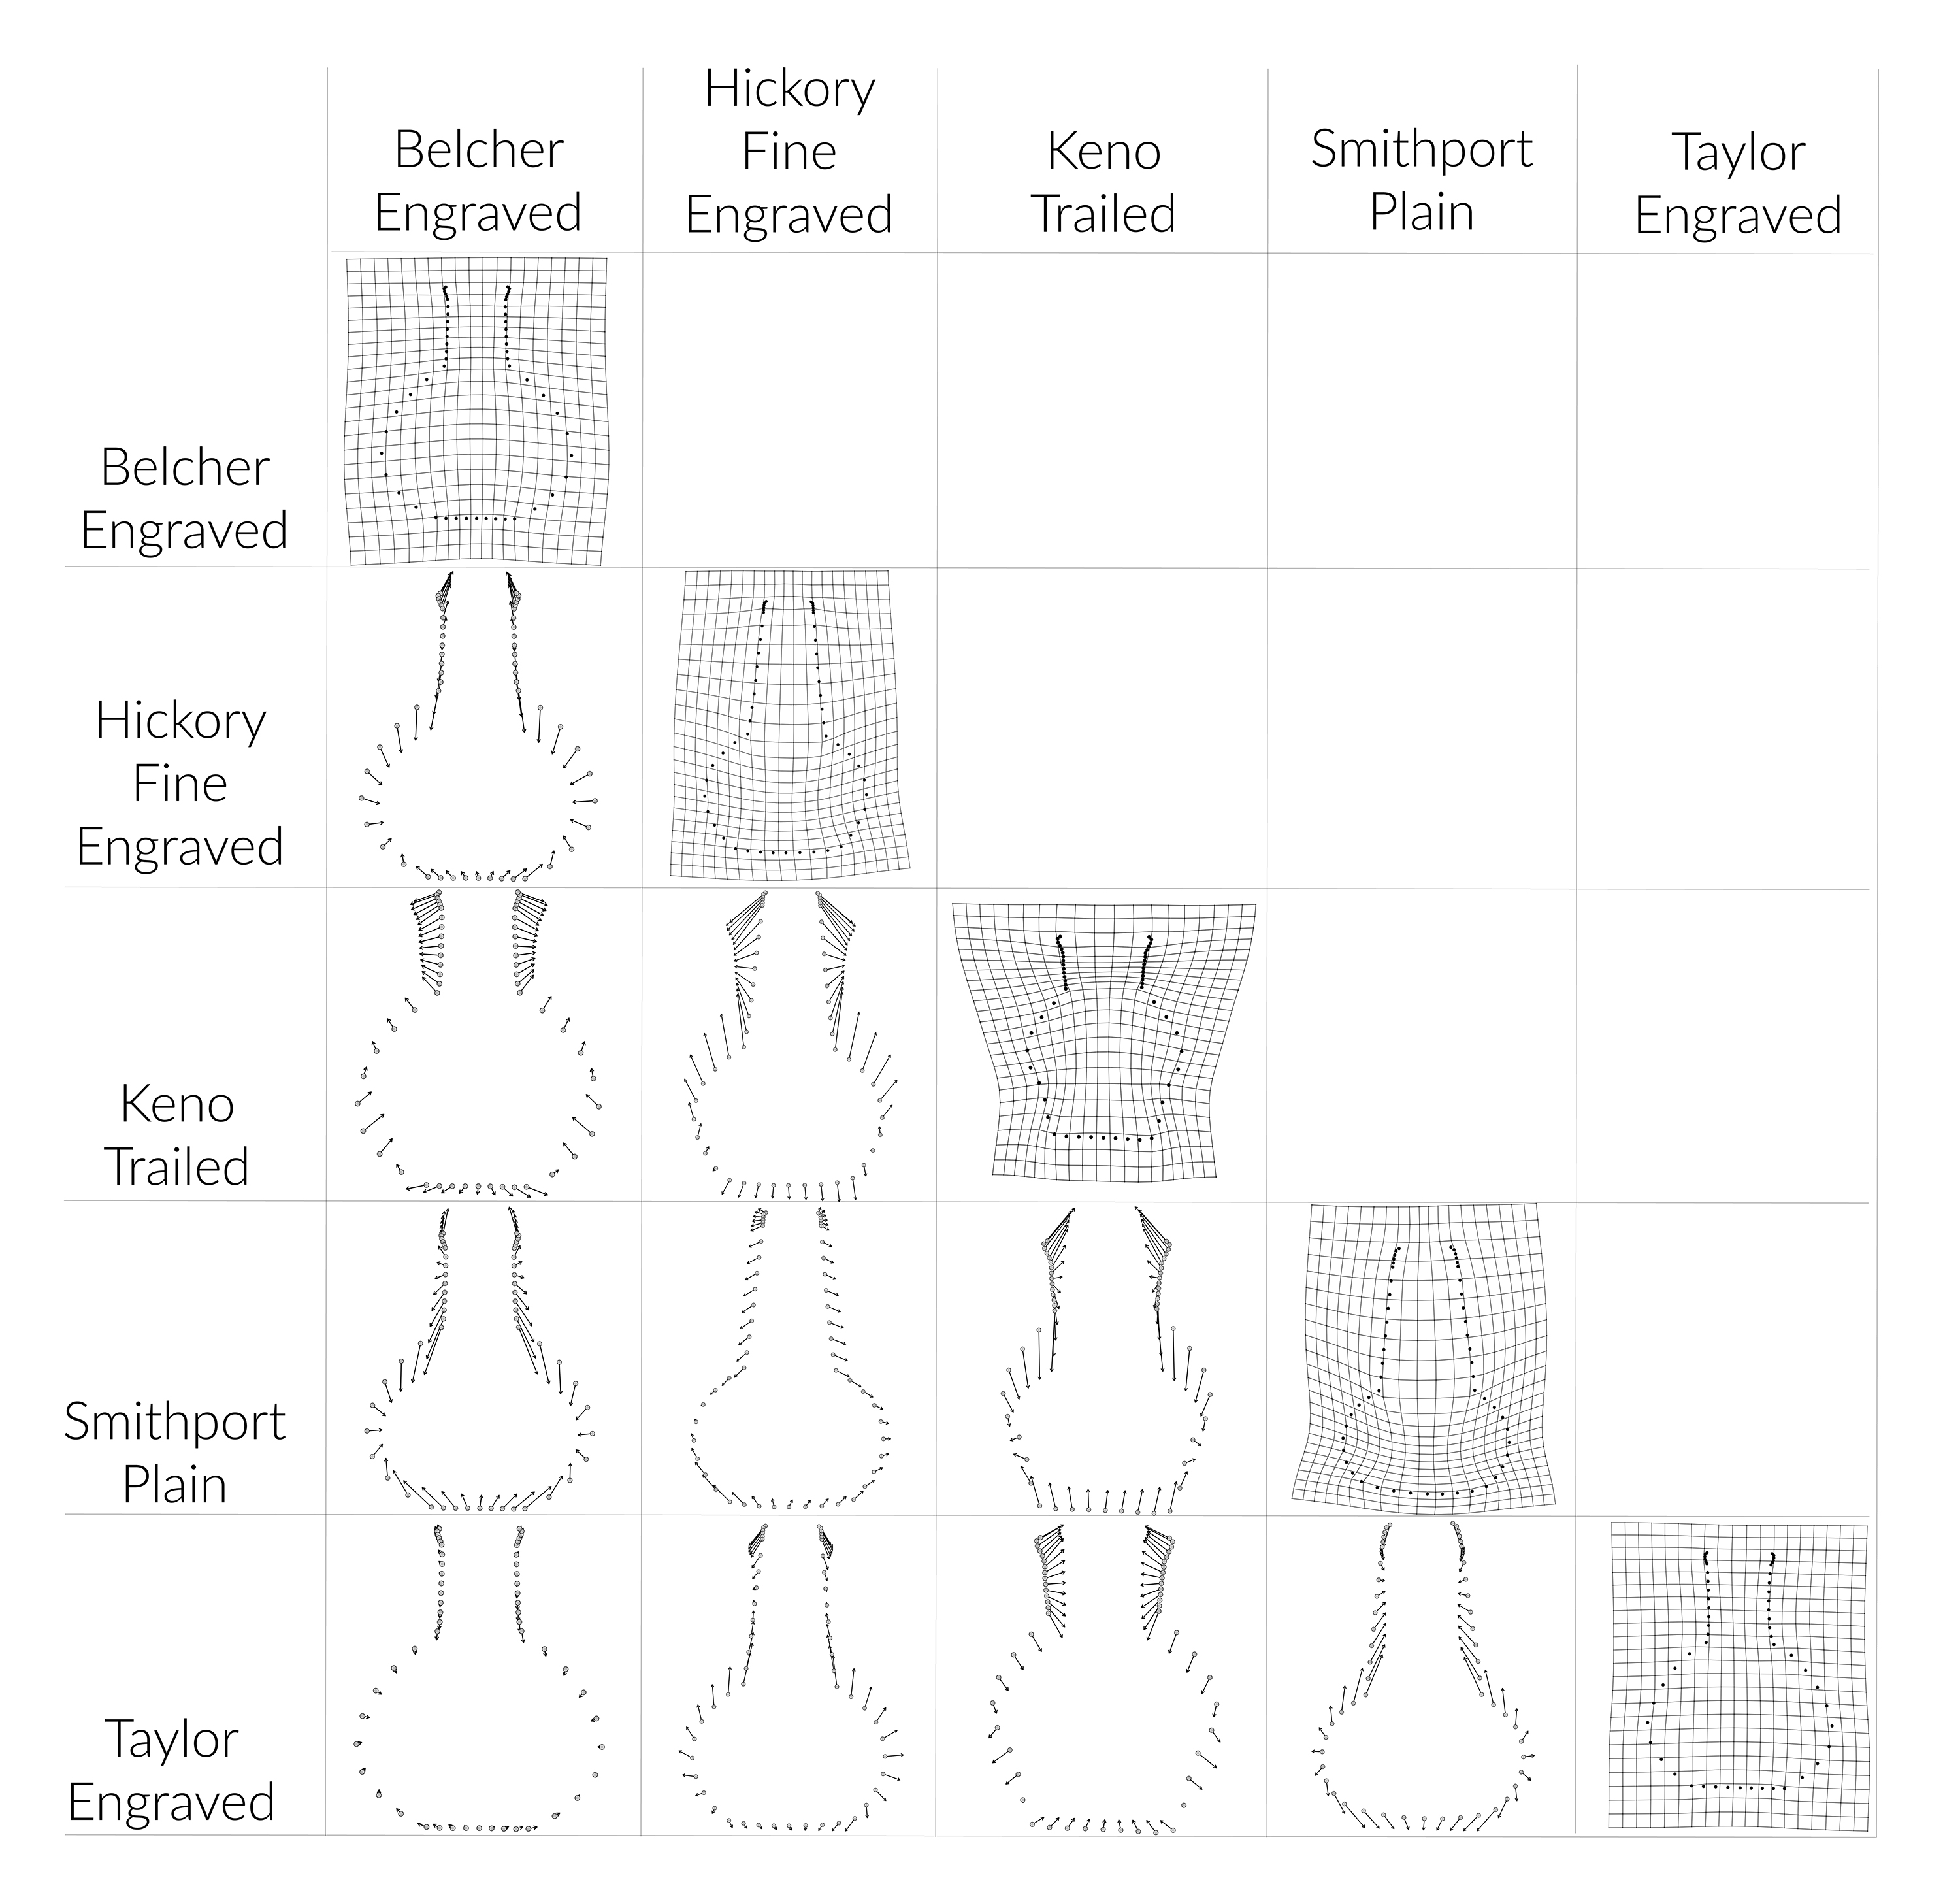
\includegraphics[width=\linewidth]{meancomp.jpg}
\caption{Comparison of mean shapes by type.}
\label{fig:FigMean}
\end{figure}

A test of morphological disparity indicates that Hickory Fine Engraved and Smithport Plain bottles display a greater range of shape variation among individuals relative to other groups, and differ significantly from the Belcher Engraved, Keno Trailed, and Taylor Engraved bottles (Table ~\ref{tab:TblDISPx}). Thus, the Formative-Early Caddo bottles encompass a greater range of morphological variability than the Late-Historic Caddo bottles in the sample. 

\begin{table}[htbp]\centering
\footnotesize
\caption{P-values and pairwise absolute differences between variances for a test of morphological disparity (RRPP = 1000).}
\centering
\begin{tabular}{lrrrrr}
\toprule
 & Belcher Eng & Hickory FE & Keno Tr & Smithport Pl & Taylor Eng\\
\midrule
Belcher Eng & 1.000 & \textbf{0.052} & 0.836 & \textbf{0.020} & 0.775\\
 & (0.0000000000) & (0.006004030) & (0.0009198292) & (0.013479467) & (0.001206460)\\
Hickory FE & \textbf{0.052} & 1.000 & 0.133 & 0.142 & 0.239\\
 & (0.0060040304) & (0.000000000) & (0.0069238596) & (0.007475437) & (0.004797570)\\
Keno Tr & 0.836 & 0.133 & 1.000 & \textbf{0.025} & 0.618\\
 & (0.0009198292) & (0.006923860) & (0.0000000000) & (0.014399297) & (0.002126289)\\
Smithport Pl & \textbf{0.020} & 0.142 & \textbf{0.025} & 1.000 & \textbf{0.034}\\
 & (0.0134794674) & (0.007475437) & (0.0143992965) & (0.000000000) & (0.012273007)\\
Taylor Eng & 0.775 & 0.239 & 0.618 & \textbf{0.034} & 1.000\\
 & (0.0012064601) & (0.004797570) & (0.0021262892) & (0.012273007) & (0.000000000)\\
\bottomrule
\end{tabular}\\
\smallskip
\textit{Significant results in bold; pairwise absolute differences between variances in parentheses.}
\label{tab:TblDISPx}
\end{table}

A test of morphological integration for the aggregated sample reveals significant integration (1000 random permutations; r-PLS = 0.883; P-value = 0.001), indicating that the discrete traits (rim, neck, body, and base) used in the manufacture of Caddo bottles vary in a coordinated manner. A pairwise test of morphological integration was used to identify which traits can be said to covary. Results indicate that for this sample of Caddo bottles, the rim and base are significantly integrated, and that the neck and body are significantly integrated (Table ~\ref{tab:Tblmorphinteg}).

\begin{table}[htbp]\centering
\footnotesize
\caption{P-values and effect sizes for morphological integration by trait (rim [A], neck [B], body [C], and base [D]) based on 1000 random permutations.}
\centering
\begin{tabular}{lcccccc}
\toprule
 & AB.int & AC.int & AD.int & BC.int & BD.int & CD.int\\
\midrule
AB.int & 1.00000000 & 0.27409817 & \textbf{0.02220463} & 0.31107177 & 0.1602111 & 0.09225511\\
	   & (0.0000000) & (0.6004651) & (2.0102073) & (0.4928147) & (0.9935906) & (1.3269954)\\
AC.int & 0.27409817 & 1.00000000 & 0.06794345 & 0.45439429 & 0.3279348 & 0.21815349\\
	   & (0.6004651) & (0.0000000) & (1.4912842) & (0.1145667) & (0.4456230) & (0.7784446)\\
AD.int & \textbf{0.02220463} & 0.06794345 & 1.00000000 & \textbf{0.05411459} & 0.1655456 & 0.24522367\\
	   & (2.0102073) & (1.4912842) & (0.0000000) & (1.6062036) & (0.9719185) & (0.6895975)\\
BC.int & 0.31107177 & 0.45439429 & \textbf{0.05411459} & 1.00000000 & 0.2897292 & 0.18639410\\
	   & (0.4928147) & (0.1145667) & (1.6062036) & (0.0000000) & (0.5541759) & (0.8912628)\\
BD.int & 0.16021110 & 0.32793480 & 0.16554555 & 0.28972922 & 1.0000000 & 0.38177146\\
	   & (0.9935906) & (0.4456230) & (0.9719185) & (0.5541759) & (0.0000000) & (0.3008316)\\
CD.int & 0.09225511 & 0.21815349 & 0.24522367 & 0.18639410 & 0.3817715 & 1.00000000\\
	   & (1.3269954) & (0.7784446) & (0.6895975) & (0.8912628) & (0.3008316) & (0.0000000)\\
\bottomrule
\end{tabular}\\
\smallskip
\textit{Significant results in bold; effect sizes for pairwise differences in PLS effect size in parentheses.}\\
\label{tab:Tblmorphinteg}
\end{table}

\subsection{Hickory Fine Engraved and Smithport Plain base/body comparison}

Visual inspection of the 10 Hickory Fine Engraved and Smithport Plain vessels indicate two distinct bottle forms for these types that occur between the southern (Allen Plantation, Gahagan Mound, and Smithport Landing) and northern (Belcher Mound) sites. To test whether a significant difference in base/body morphology exists between the two forms, the Hickory Fine Engraved and Smithport Plain bottles from the previous analysis were analysed with two additional Smithport Plain vessels (Webb 405 and 430) from Burials 11 and 12 at the Belcher Mound site (both with broken necks) (see also Table ~\ref{tab:Tbl1}). A subset (base and body) of the same landmarks and equidistant semilandmark configuration used in the previous analysis (landmarks/semilandmarks 15-41) were also used in this test, since the two additional samples are missing sections of the neck and rim. The mean consensus configuration and Procrustes residuals were calculated using a generalised Procrustes analysis (GPA) for the aggregated sample (Figure ~\ref{fig:FigGPAbba}). 

\begin{figure}[htbp]\centering
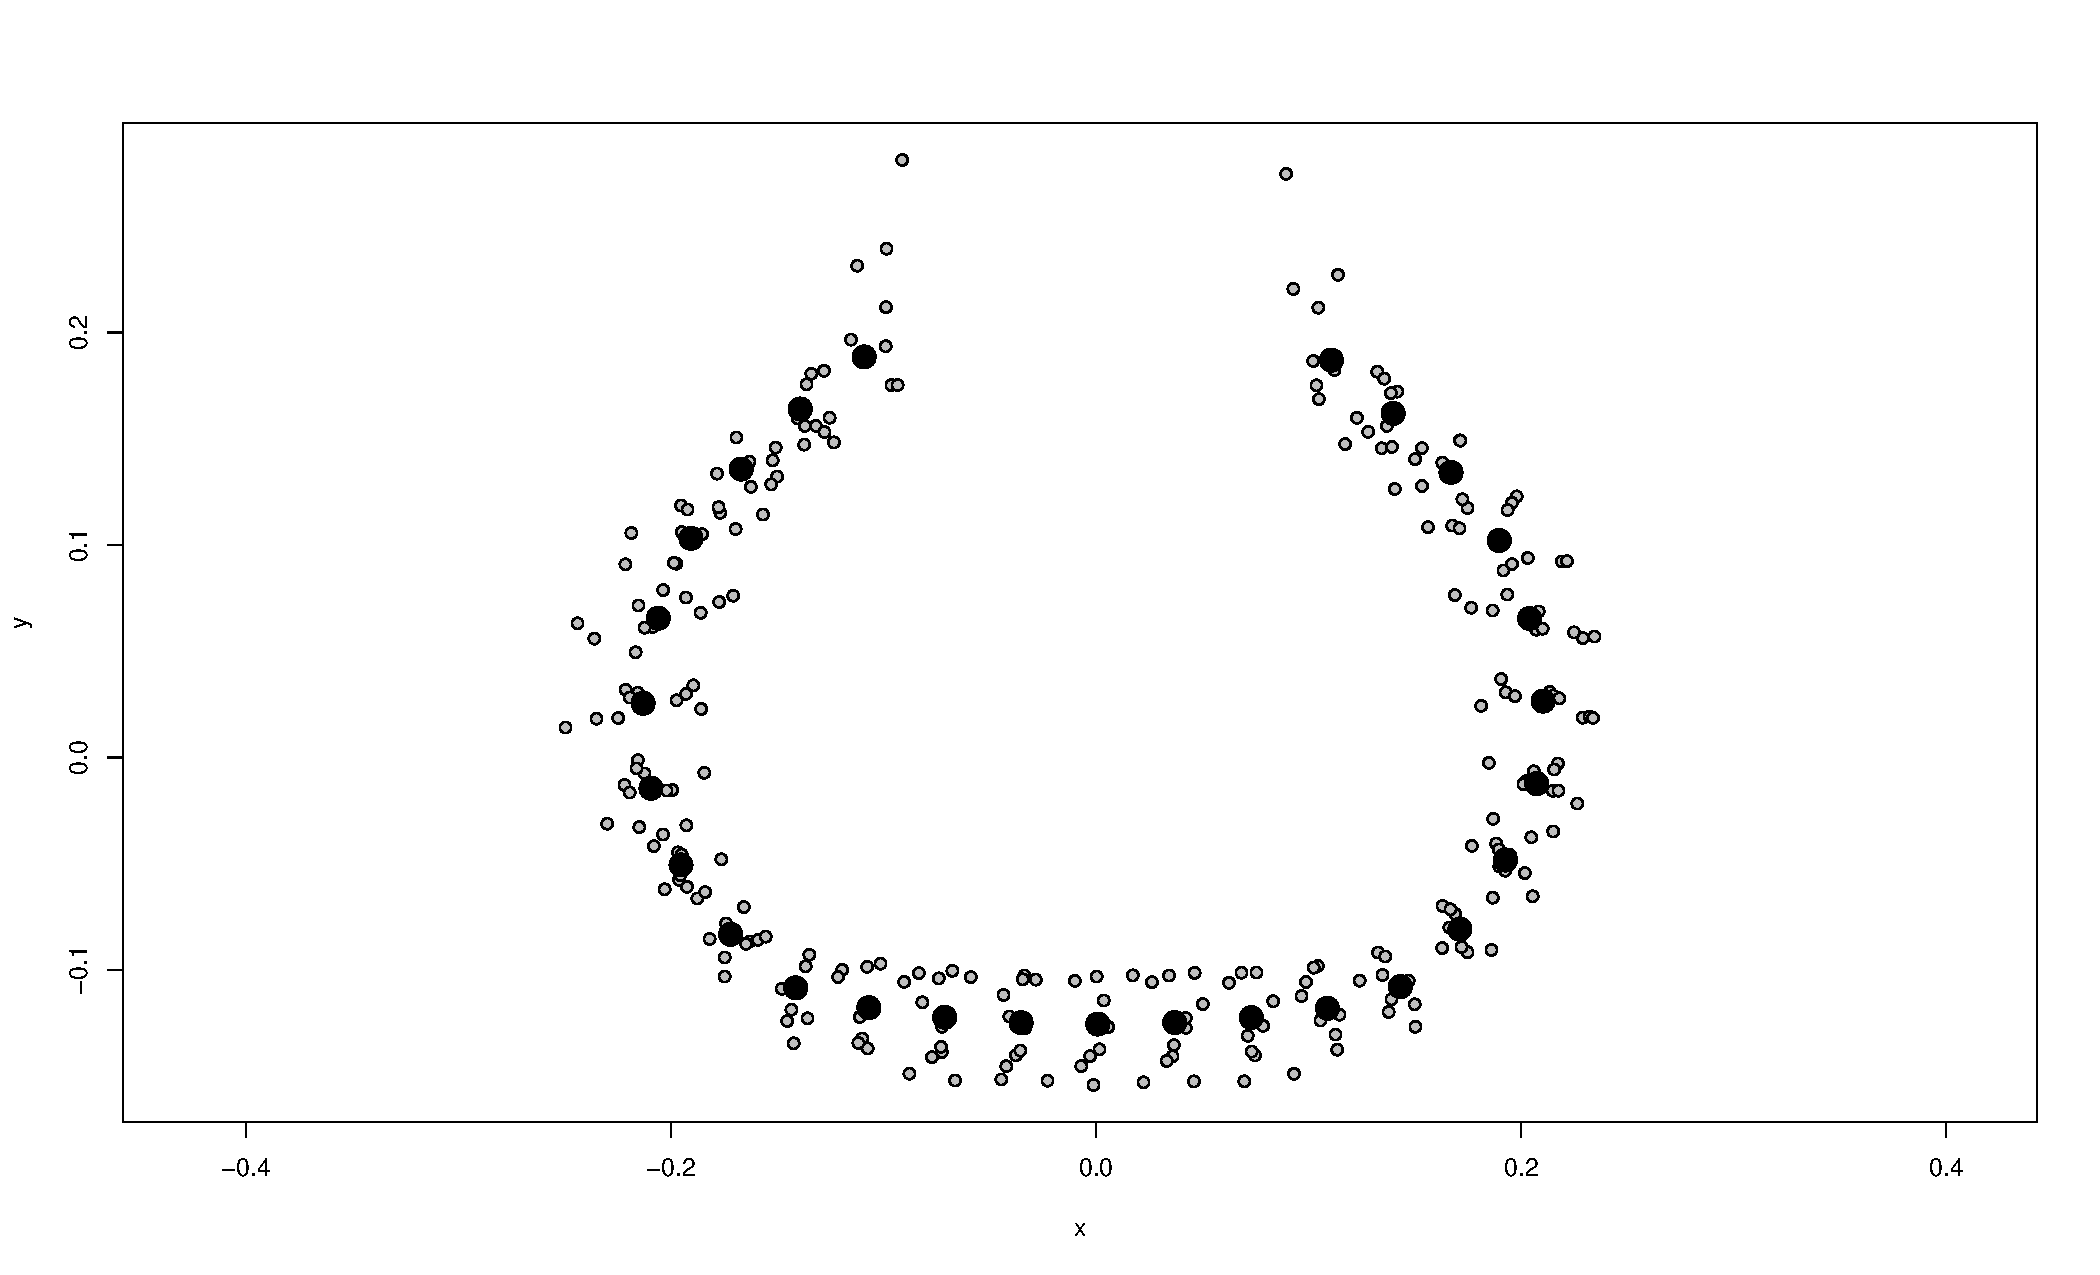
\includegraphics[width=\linewidth]{gpa-bba}
\caption{Results of Generalized Procrustes Analysis for the base/body sample. Mean consensus configuration shown in black; samples in gray.}
\label{fig:FigGPAbba}
\end{figure}

Principal components analysis (PCA) was conducted on scaled, translated, and rotated landmarks, and demonstrate that the first two PCs account for 78 (PC1) and 14 (PC2) percent of the variation in bottle body/base shape (Table ~\ref{tab:Tbl2} and Figure ~\ref{fig:FigPCA}). Together, PC1 and PC2 account for 92 percent of shape variation for base/body shape, with all remaining PCs representing less than three percent of the variation (Table ~\ref{tab:Tbl2}). The first two PCs are plotted in Figure ~\ref{fig:FigPCA}, where warp grids represent the shape changes along PC1. This plot indicates that shape changes associated with PC1 articulate most readily with height. Those shape changes associated with PC2 are dominated by differences in bottle width.

\begin{table}[htbp]\centering
\footnotesize
\caption{Results of principal components analysis for the nine PCs (100 percent of total variance explained).}
\centering
\begin{tabular}{lp{2cm}p{2cm}p{2cm}}
\toprule
 & SD & PVE & CVE\\
\midrule
PC1 & 0.1261 & 0.7788 & 0.7788\\
PC2 & 0.05324 & 0.13876 & 0.91755\\
PC3 & 0.02849 & 0.03975 & 0.95730\\
PC4 & 0.02473 & 0.02994 & 0.98724\\
PC5 & 0.01134 & 0.00630 & 0.99354\\
PC6 & 0.007987 & 0.003120 & 0.996660\\
PC7 & 0.005782 & 0.001640 & 0.998300\\
PC8 & 0.005365 & 0.001410 & 0.999710\\
PC9 & 0.00244 & 0.00029 & 1.00000\\
\bottomrule
\end{tabular}
\smallskip\\
SD - standard deviation; PVE - percentage variance explained; CVE - cumulative variance explained.
\label{tab:Tbl2}
\end{table}

\begin{figure}[htbp]\centering
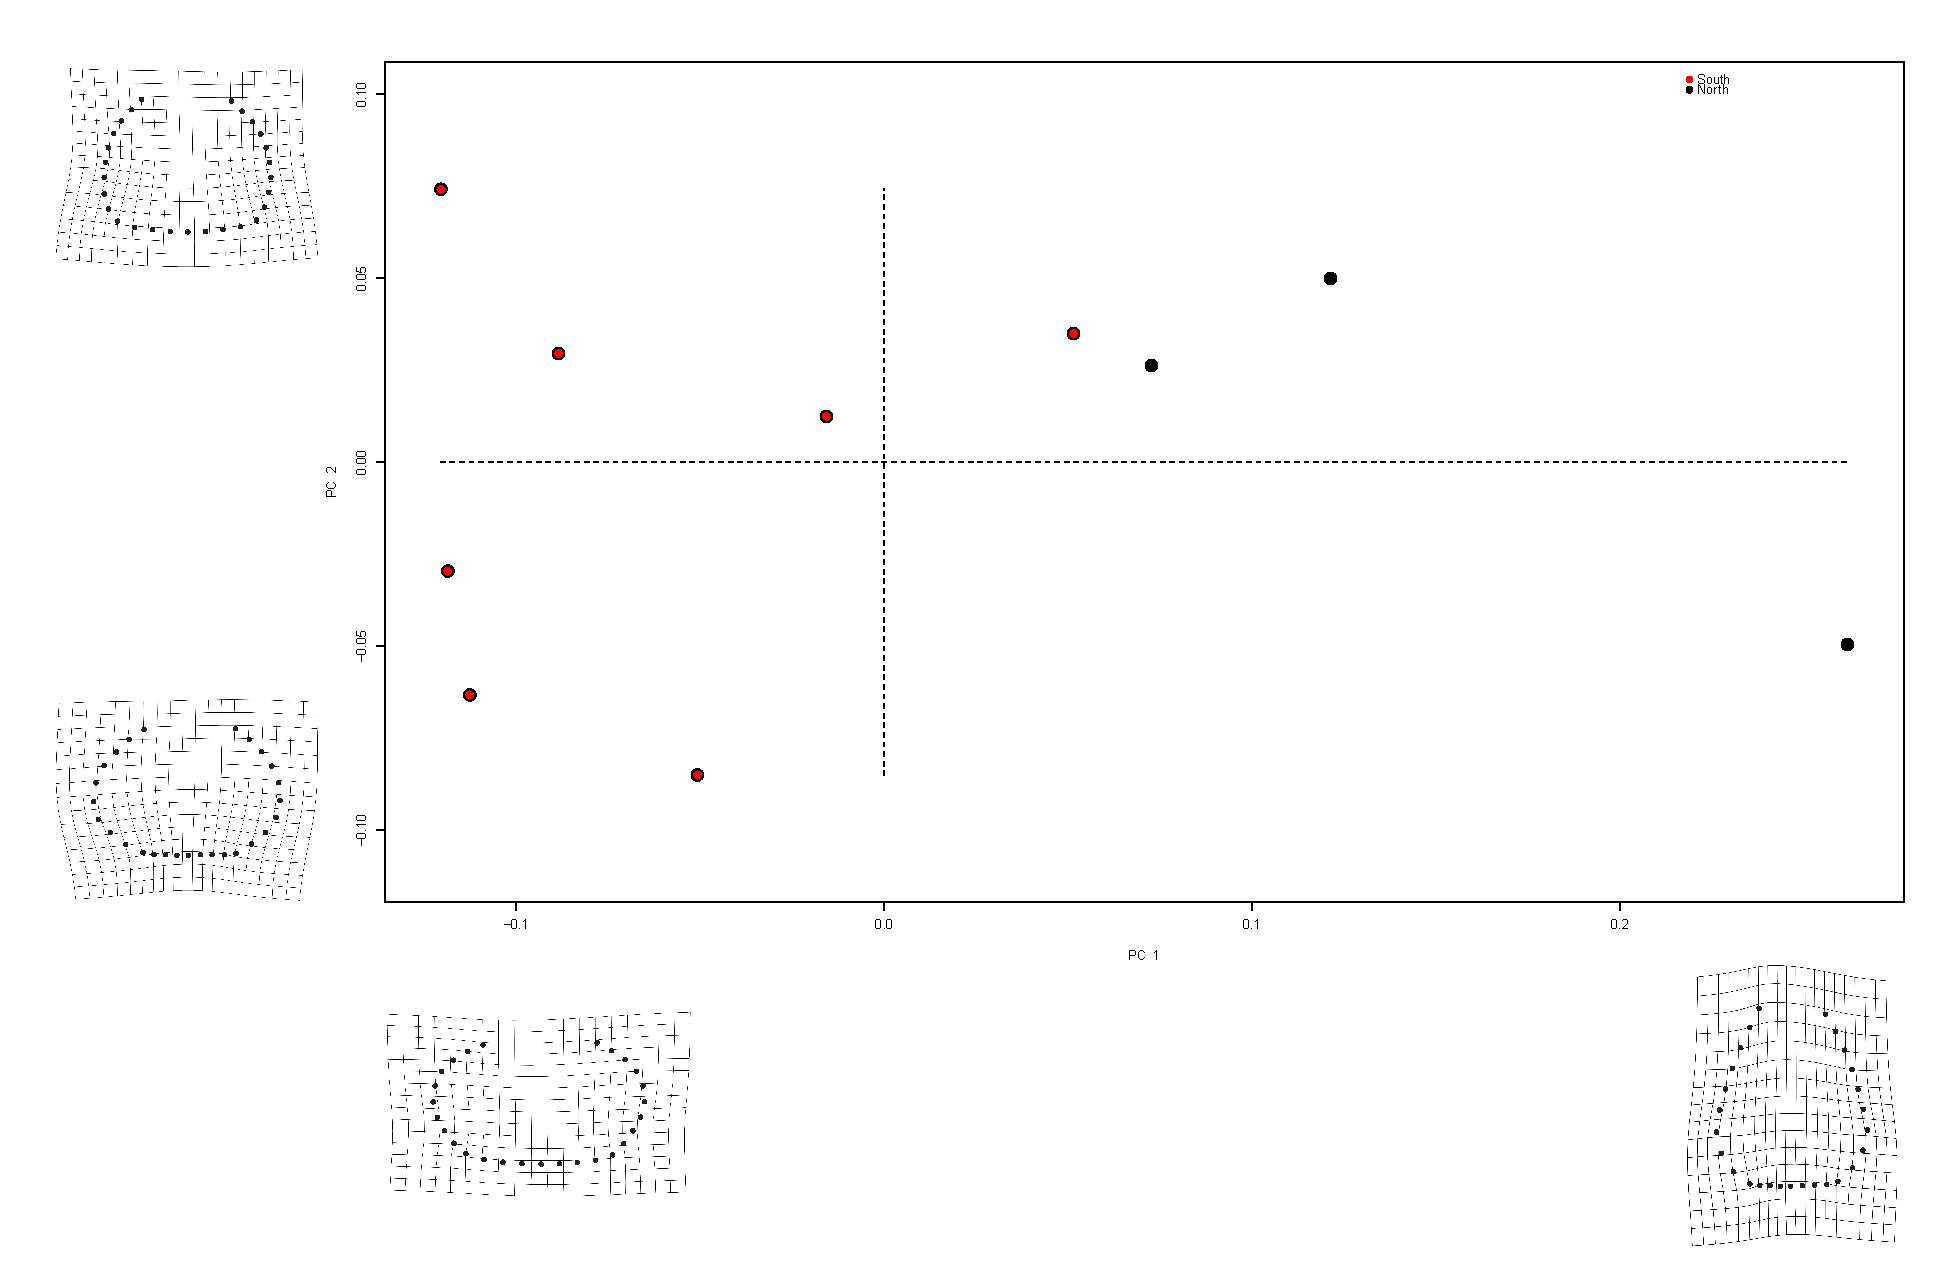
\includegraphics[width=\linewidth]{pcabba}
\caption{Principal components analysis for Hickory Fine Engraved and Smithport Plain base/body analysis segregated by North-South groups.}
\label{fig:FigPCAbba}
\end{figure}

A Procrustes ANOVA was used to test for a significant difference in allometry. Results of the ANOVA indicate that allometry in the sample is not significant. A second Procrustes ANOVA was used to test for a significant difference between the two types. Results of the ANOVA indicate that the base/body of the Hickory Fine Engraved and Smithport Plain types do not differ significantly. A third Procrustes ANOVA was used to test for a significant difference in bottle shape by group (North or South). Results of the ANOVA indicate a significant difference in bottle shape by group (RRPP = 1000; Rsq = 0.54538; Pr(>F) = 0.0085). A pairwise test of shapes was subsequently conducted for groups designated by group (North or South). Results confirm a significant difference in bottle base/body shape between the Hickory Fine Engraved and Smithport Plain bottles produced at the Belcher Mound site (North) when compared with bottles produced at the Allen Plantation, Gahagan Mound, and Smithport Landing sites (South) (Table ~\ref{tab:Tblpairbba}).

\begin{table}[htbp]\centering
\footnotesize
\caption{P-values and effect sizes for advanced Procrustes ANOVA and pairwise test (RRPP = 1000) of shape by group (North and South).}
\centering
\begin{tabular}{lrr}
\toprule
 & North & South\\
\midrule
North & 1.00 & \textbf{0.01}\\
 & (0.000000) & (3.141828)\\
South & \textbf{0.01} & 1.00\\
 & (3.141828) & (0.000000)\\
\bottomrule
\end{tabular}\\
\smallskip
\textit{Significant results in bold; effect sizes (z) listed in parentheses.}
\label{tab:Tblpairbba}
\end{table}

\section{Discussion and Conclusion}

This repository-based analysis of a curated and majority-NAGPRA collection of intact or reconstructed Caddo bottles resulted in the identification of similarities, differences, and a general trend toward standardisation for the aggregated sample. Specifically, it resulted in the identification of morphological disparity between Formative-Early and Late-Historic Caddo ceramics, identification and clarification of morphological similarities between Hickory Fine Engraved and Smithport Plain bottle shapes, identification and clarification of morphological similarities between Belcher Engraved and Taylor Engraved bottle shapes, identification of significant morphological integration in the whole vessel sample, and the identification of two discrete (tentatively north-south) bottle shapes for the Hickory Fine Engraved and Smithport Plain vessels from northwest Louisiana. 

The analysis of morphological disparity yielded a significant difference between Formative-Early and Late-Historic Caddo bottle shapes, demonstrating that Formative-Early Caddo bottles occupy a greater range of morphospace than Late-Historic Caddo bottles in the sample. While further work is warranted, these results provide evidence that may support an argument for the gradual standardisation of Caddo bottle shapes through time. Whether, and to what extent, that trend may articulate with a potential shift toward craft specialisation is currently unknown. The test of allometry indicates significantly divergent trajectories between Formative-Early and Late-Historic Caddo bottles, and those bottles that do not differ significantly in shape do express differing allometric trajectories. These results also indicate---although based upon a small sample---that Formative-Early bottles extended into a larger size range. 

While not explored here, this line of evidence may prove useful in discussions of standardisation \citep{RN11631} couched within examinations of craft specialisation \citep{RN29,RN250,RN28,RN18,RN1989}. Certainly craft specialisation is not the only theoretical construct that has utility here, and results might also be expressed in discussions of communities of practice and identity (sensu \citet{RN11666} and \citet{RN11602}), or a wide range of additional approaches; however, the bulk of current archaeological applications of GM enlist evolutionary archaeology \citep{RN1742,RN11779}. 

The shape of Hickory (Fine) Engraved and Smithport Plain bottles in this sample do not differ significantly, and two distinct bottle shapes were found to occur in that population. It is worth noting that the difference in bottle morphology is more dramatic for the Smithport Plain bottles, and the Hickory Fine Engraved shapes may provide clarification regarding a possible morphological transition that occurred across the two types (Figure ~\ref{fig:FigPCAbba}). While the north-south difference is significant for this sample, the northern sample is informed by a single site (Belcher Mound). The addition of vessels from other areas of the Southern Caddo Area will aid in the continued refinement of those results presented here. More work is needed to better characterise the variation in shape for these bottle types, and to identify the potential shifts in social practices that articulate with the variations in bottle morphology.

The test of morphological integration for the Caddo bottle sample was significant, meaning that the different components of the bottles (rim, neck, base, and body) vary in a coordinated manner. Further, those traits associated with the rim and base are significantly integrated, as are those associated with the neck and body. Although preliminary, this result provides support for the hypothesis that Caddo potters were adhering to a template of vessel shape associated with specific decorative motifs \citep{RN1660}. It also adds to it by clarifying which of the discrete morphological traits can be said to covary. This information further elucidates upon questions of production, highlights those components of the vessel that covary, and has utility for efforts to conceptually (or physically) reconstruct missing components of fragmented Caddo bottles. 

Comparative studies of vessel morphology are necessary to expound upon the complexities of the ceramic shapes employed by Caddo potters. This example enlists an aggregated sample of Caddo bottles paired with a suite of qualitative data produced by the original investigator. The addition of GM tools provides a method of integrating qualitative attributes (temper, firing, decorative method, motif, etc.) with morphological data to test for significant relationships. That information, in turn, is a valuable contribution to a wide range of potential interpretations that include the evolution of design and morphology, craft production, the identification of communities of practice and identity, as well as many others.

In addition to their analytical value, those 3D data produced throughout the course of this study have been repurposed as a tool for public archaeology, citizen science, and general outreach. While not all of the bottles have been added, many can be viewed on Sketchfab, and selected vessels are available for download on Zenodo @ CERN. The scans are also being repurposed to test and refine settings on a 3D printer to ensure that the morphology of the printed specimens is as close to the original as possible (Figure ~\ref{fig:FigEffigy}), providing a means of interacting with an accurate proxy while reducing physical access to the original specimen. Further still, should the Caddo Nation of Oklahoma decide to repatriate this collection, the 3D meshes would remain a valuable tool for comparative analyses long after the originals had been repatriated and reburied. 

\begin{figure}[ht]\centering
\includegraphics[width=\linewidth]{figeffigy}
\caption{Computer-aided inspection of the original 3D scan data contrasted with a scan of a 3D print of the same object. This Caddo effigy vessel is a part of the Webb collection, and comes from the Belcher Mound in northwest Louisiana.}
\label{fig:FigEffigy}
\end{figure}

The progression of this analysis will include (1) an expansion of the Hickory (Fine) Engraved and Smithport Plain analysis to explore whether it may be possible to identify the locus of innovation associated with the two bottle shapes found here, as well as whether other bottle shapes that were employed by the Caddo makers of these types, (2) an expansion of the Belcher and Taylor Engraved sample to test whether the similarity in bottle shape identified in this study is localised, (3) continued analyses of morphological disparity among different temporal periods (Formative, Early, Middle, Late, and Historic) to test whether significant morphological disparity and size variation between these time periods varies elsewhere across time and space, and (4) the continued use of morphological integration to identify which morphological traits associated with Caddo bottle manufacture might be said to covary. The application of GM methods to questions of Caddo ceramic morphology can produce meaningful results that contribute to the interpretation of Caddo sites, communities, and the possible relationships that existed between them, while simultaneously providing a systematic and rigorous method that archaeologists can use to test a wide range of previous, current, and future hypotheses. Those results presented here provide a preview of that utility, and serve as the foundation for the progression and logical expansion of this research design. 

\section*{Acknowledgments}

I extend my gratitude to the Caddo Nation of Oklahoma, the Williamson Museum at Northwestern State University (Hiram F. [Pete] Gregory and Jeffrey R. Girard), the Louisiana State Exhibit Museum (Nita Cole), and the LSU Museum of Natural Science (Rebbecca A. Saunders and Beverly S. Nuschler) for the requisite permissions and access needed to generate the 3D scans of the Caddo bottles from the Webb collection. Thanks also to Dean C. Adams, Emma Sherratt, Stephen J. Lycett, Michael J. Shott, Timothy K. Perttula, and Kersten Bergstrom for their constructive criticisms, comments, and suggestions throughout the development of this research design, and to the anonymous reviewers whose comments further improved the manuscript. Development of this analytical work flow and the production of 3D scans from the Clarence H. Webb collection was funded by a grant to RZS (P14AP00138) from the National Center for Preservation Technology and Training.

\section*{References Cited}

\bibliography{mybibfile}

\end{document}